\documentclass[12pt, a4paper]{article}\usepackage[]{graphicx}\usepackage[]{xcolor}
% maxwidth is the original width if it is less than linewidth
% otherwise use linewidth (to make sure the graphics do not exceed the margin)
\makeatletter
\def\maxwidth{ %
  \ifdim\Gin@nat@width>\linewidth
    \linewidth
  \else
    \Gin@nat@width
  \fi
}
\makeatother

\definecolor{fgcolor}{rgb}{0.345, 0.345, 0.345}
\newcommand{\hlnum}[1]{\textcolor[rgb]{0.686,0.059,0.569}{#1}}%
\newcommand{\hlstr}[1]{\textcolor[rgb]{0.192,0.494,0.8}{#1}}%
\newcommand{\hlcom}[1]{\textcolor[rgb]{0.678,0.584,0.686}{\textit{#1}}}%
\newcommand{\hlopt}[1]{\textcolor[rgb]{0,0,0}{#1}}%
\newcommand{\hlstd}[1]{\textcolor[rgb]{0.345,0.345,0.345}{#1}}%
\newcommand{\hlkwa}[1]{\textcolor[rgb]{0.161,0.373,0.58}{\textbf{#1}}}%
\newcommand{\hlkwb}[1]{\textcolor[rgb]{0.69,0.353,0.396}{#1}}%
\newcommand{\hlkwc}[1]{\textcolor[rgb]{0.333,0.667,0.333}{#1}}%
\newcommand{\hlkwd}[1]{\textcolor[rgb]{0.737,0.353,0.396}{\textbf{#1}}}%
\let\hlipl\hlkwb

\usepackage{framed}
\makeatletter
\newenvironment{kframe}{%
 \def\at@end@of@kframe{}%
 \ifinner\ifhmode%
  \def\at@end@of@kframe{\end{minipage}}%
  \begin{minipage}{\columnwidth}%
 \fi\fi%
 \def\FrameCommand##1{\hskip\@totalleftmargin \hskip-\fboxsep
 \colorbox{shadecolor}{##1}\hskip-\fboxsep
     % There is no \\@totalrightmargin, so:
     \hskip-\linewidth \hskip-\@totalleftmargin \hskip\columnwidth}%
 \MakeFramed {\advance\hsize-\width
   \@totalleftmargin\z@ \linewidth\hsize
   \@setminipage}}%
 {\par\unskip\endMakeFramed%
 \at@end@of@kframe}
\makeatother

\definecolor{shadecolor}{rgb}{.97, .97, .97}
\definecolor{messagecolor}{rgb}{0, 0, 0}
\definecolor{warningcolor}{rgb}{1, 0, 1}
\definecolor{errorcolor}{rgb}{1, 0, 0}
\newenvironment{knitrout}{}{} % an empty environment to be redefined in TeX

\usepackage{alltt}

%%%%%%%%%%%%%%%%%%%%%%%%%%%%%%%%%%%%%%%%%%%%%%%%%%%%%%%%%%%%%%%%

\usepackage[OT4]{polski}
\usepackage[utf8]{inputenc}
\usepackage[top=2.5cm, bottom=2.5cm, left=2cm, right=2cm]{geometry}
\usepackage{graphicx}
\usepackage{float}
\usepackage[colorlinks=true, linkcolor=blue]{hyperref}
\usepackage[polish]{babel}
\usepackage{amsmath}


%%%%%%%%%%%%%%%%%%%%%%%%%%%%%%%%%%%%%%%%%%%%%%%%%%%%%%%%%%%%%%%%



\IfFileExists{upquote.sty}{\usepackage{upquote}}{}
\begin{document}



%%%%%%%%%%%%%%%%%%%%%%%%%%%%%%%%%%%%%%%%%%%%%%%%%%%%%%%%%%%%%%%%

\title{Telco Customer Churn}
\author{Stanisław Olek}
\maketitle
\tableofcontents

\section{Wprowadzenie}

Niniejszy raport przedstawia analizę danych dotyczących rezygnacji klientów z usług telekomunikacyjnych (customer churn). Zrozumienie czynników wpływających na decyzję klientów o rezygnacji z usług jest kluczowe dla firm telekomunikacyjnych, ponieważ pozwala im opracować strategie utrzymania klientów.

\section{Wczytanie i przygotowanie danych}

\begin{knitrout}
\definecolor{shadecolor}{rgb}{0.969, 0.969, 0.969}\color{fgcolor}\begin{kframe}
\begin{alltt}
\hlcom{# wczytanie zbioru danych}
\hlstd{dane} \hlkwb{<-} \hlkwd{read.csv}\hlstd{(}
  \hlstr{'/Users/cj/Documents/ED/1/WA_Fn-UseC_-Telco-Customer-Churn.csv'}\hlstd{,}
  \hlkwc{stringsAsFactors}\hlstd{=}\hlnum{TRUE}\hlstd{)}
\end{alltt}
\end{kframe}
\end{knitrout}

\begin{knitrout}
\definecolor{shadecolor}{rgb}{0.969, 0.969, 0.969}\color{fgcolor}\begin{kframe}
\begin{alltt}
\hlstd{dane}\hlopt{$}\hlstd{SeniorCitizen} \hlkwb{<-} \hlkwd{as.factor}\hlstd{(dane}\hlopt{$}\hlstd{SeniorCitizen)}
\end{alltt}
\end{kframe}
\end{knitrout}

Po konwersji zmienna \texttt{SeniorCitizen} jest poprawnie traktowana jako zmienna jakościowa (factor), co odpowiada jej naturze, zmienna ta wskazuje bowiem, czy klient jest seniorem \texttt{1} czy nie \texttt{0}.

\subsection{Rozmiar danych}
\begin{knitrout}
\definecolor{shadecolor}{rgb}{0.969, 0.969, 0.969}\color{fgcolor}\begin{kframe}
\begin{alltt}
\hlcom{# sprawdzenie rozmiaru danych}
\hlkwd{dim}\hlstd{(dane)}
\end{alltt}
\begin{verbatim}
## [1] 7043   21
\end{verbatim}
\end{kframe}
\end{knitrout}


Zbiór danych składa się z 7043 przypadków (wierszy) oraz 21 cech (kolumn)

\subsection{Typy poszczególnych cech}



\paragraph{Zmienne jakościowe (factor):}
\begin{itemize}
\item customerID, \item gender, \item SeniorCitizen, \item Partner, \item Dependents, \item PhoneService, \item MultipleLines, \item InternetService, \item OnlineSecurity, \item OnlineBackup, \item DeviceProtection, \item TechSupport, \item StreamingTV, \item StreamingMovies, \item Contract, \item PaperlessBilling, \item PaymentMethod, \item Churn
\end{itemize}
Liczba zmiennych jakościowych: 18

\paragraph{Zmienne ilościowe (numeric):}
\begin{itemize}
\item tenure, \item MonthlyCharges, \item TotalCharges
\end{itemize}
Liczba zmiennych ilościowych: 3


\subsection{Przydatność cech}
W danych występuje cecha \texttt{customerID}, która pełni rolę identyfikatora klientów. Cecha ta nie wnosi wartości merytorycznej do analizy, dlatego należy ją usunąć przed dalszą analizą.

\begin{knitrout}
\definecolor{shadecolor}{rgb}{0.969, 0.969, 0.969}\color{fgcolor}\begin{kframe}
\begin{alltt}
\hlcom{# usunięcie kolumny customerID}
\hlstd{dane} \hlkwb{<-} \hlstd{dane[,}\hlopt{-}\hlnum{1}\hlstd{]}

\hlcom{# sprawdzenie struktury danych po usunięciu kolumny customerID}
\hlkwd{dim}\hlstd{(dane)}
\end{alltt}
\begin{verbatim}
## [1] 7043   20
\end{verbatim}
\end{kframe}
\end{knitrout}


\newpage
\subsection{Brakujące obserwacje}
\begin{knitrout}
\definecolor{shadecolor}{rgb}{0.969, 0.969, 0.969}\color{fgcolor}\begin{kframe}
\begin{alltt}
\hlcom{# sprawdzenie czy w danych występują brakujące wartości (NA)}
\hlkwd{sum}\hlstd{(}\hlkwd{is.na}\hlstd{(dane))}
\end{alltt}
\begin{verbatim}
## [1] 11
\end{verbatim}
\begin{alltt}
\hlcom{# sprawdzenie liczby brakujących wartości dla każdej cechy}
\hlstd{na_licznik} \hlkwb{<-} \hlkwd{sapply}\hlstd{(dane,} \hlkwa{function}\hlstd{(}\hlkwc{x}\hlstd{)} \hlkwd{sum}\hlstd{(}\hlkwd{is.na}\hlstd{(x)))}
\hlstd{na_licznik}
\end{alltt}
\begin{verbatim}
##           gender    SeniorCitizen          Partner       Dependents 
##                0                0                0                0 
##           tenure     PhoneService    MultipleLines  InternetService 
##                0                0                0                0 
##   OnlineSecurity     OnlineBackup DeviceProtection      TechSupport 
##                0                0                0                0 
##      StreamingTV  StreamingMovies         Contract PaperlessBilling 
##                0                0                0                0 
##    PaymentMethod   MonthlyCharges     TotalCharges            Churn 
##                0                0               11                0
\end{verbatim}
\end{kframe}
\end{knitrout}

W danych występuje 11 brakujących wartości, wszystkie w kolumnie \texttt{TotalCharges}. Brakujące wartości są kodowane jako \texttt{NA} w R.


\subsection{Nietypowe wartości}

\begin{knitrout}
\definecolor{shadecolor}{rgb}{0.969, 0.969, 0.969}\color{fgcolor}\begin{kframe}
\begin{alltt}
\hlcom{# sprawdzenie czy zmienne numeryczne zawierają nietypowe wartości}
\hlkwd{summary}\hlstd{(dane[, numeric_zmienne])}
\end{alltt}
\begin{verbatim}
##      tenure      MonthlyCharges    TotalCharges   
##  Min.   : 0.00   Min.   : 18.25   Min.   :  18.8  
##  1st Qu.: 9.00   1st Qu.: 35.50   1st Qu.: 401.4  
##  Median :29.00   Median : 70.35   Median :1397.5  
##  Mean   :32.37   Mean   : 64.76   Mean   :2283.3  
##  3rd Qu.:55.00   3rd Qu.: 89.85   3rd Qu.:3794.7  
##  Max.   :72.00   Max.   :118.75   Max.   :8684.8  
##                                   NA's   :11
\end{verbatim}
\begin{alltt}
\hlcom{# sprawdzenie czy wartości TotalCharges = NA mają związek z tenure}
\hlstd{dane}\hlopt{$}\hlstd{tenure[}\hlkwd{is.na}\hlstd{(dane}\hlopt{$}\hlstd{TotalCharges)]}
\end{alltt}
\begin{verbatim}
##  [1] 0 0 0 0 0 0 0 0 0 0 0
\end{verbatim}
\begin{alltt}
\hlcom{# sprawdzenie, czy występują nietypowe wartości w zmiennych jakościowych }
\hlkwa{for} \hlstd{(col} \hlkwa{in} \hlkwd{names}\hlstd{(dane)[}\hlkwd{sapply}\hlstd{(dane, is.factor)]) \{}
  \hlstd{unikalne_wartosci} \hlkwb{<-} \hlkwd{unique}\hlstd{(}\hlkwd{as.character}\hlstd{(dane[[col]]))}
  \hlstd{nietypowe} \hlkwb{<-} \hlstd{unikalne_wartosci[}
    \hlstd{unikalne_wartosci} \hlopt \hlkwd{c}\hlstd{(}\hlstr{""}\hlstd{,} \hlstr{" "}\hlstd{,} \hlstr{"unknown"}\hlstd{,} \hlstr{"N/A"}\hlstd{,} \hlstr{"NA"}\hlstd{,} \hlstr{"-"}\hlstd{,} \hlstr{"?"}\hlstd{)]}
\hlstd{\}}

\hlkwd{length}\hlstd{(nietypowe)}
\end{alltt}
\begin{verbatim}
## [1] 0
\end{verbatim}
\end{kframe}
\end{knitrout}

Wszystkie wiersze z brakującymi wartościami w kolumnie \texttt{TotalCharges} mają wartość 0 w kolumnie \texttt{tenure}. Sugeruje to, że brakujące wartości \texttt{TotalCharges} dotyczą nowych klientów, którzy nie dokonali jeszcze żadnych płatności.
Nie zaobserwowano innych nietypowych wartości czy niestandardowego kodowania brakujących danych w danych.







\newpage
\section{Analiza zmiennych ilościowych}

\subsection{Analiza dla zbioru bez podziału na grupy}

\subsubsection{Podstawowe wskaźniki sumaryczne}
% latex table generated in R 4.3.2 by xtable 1.8-4 package
% Tue Apr  1 01:14:35 2025
\begin{table}[ht]
\centering
\caption{Podstawowe statystyki dla zmiennych ilościowych} 
\label{tab:stats_all}
\begin{tabular}{rrrr}
  \hline
 & tenure & MonthlyCharges & TotalCharges \\ 
  \hline
Średnia & 32.37 & 64.76 & 2283.30 \\ 
  Mediana & 29.00 & 70.35 & 1397.47 \\ 
  Min & 0.00 & 18.25 & 18.80 \\ 
  Max & 72.00 & 118.75 & 8684.80 \\ 
  Q1.25\% & 9.00 & 35.50 & 401.45 \\ 
  Q3.75\% & 55.00 & 89.85 & 3794.74 \\ 
  SD & 24.56 & 30.09 & 2266.77 \\ 
  IQR & 46.00 & 54.35 & 3393.29 \\ 
   \hline
\end{tabular}
\end{table}


\newpage
\subsubsection{Histogramy}
\begin{knitrout}
\definecolor{shadecolor}{rgb}{0.969, 0.969, 0.969}\color{fgcolor}\begin{figure}[H]

{\centering 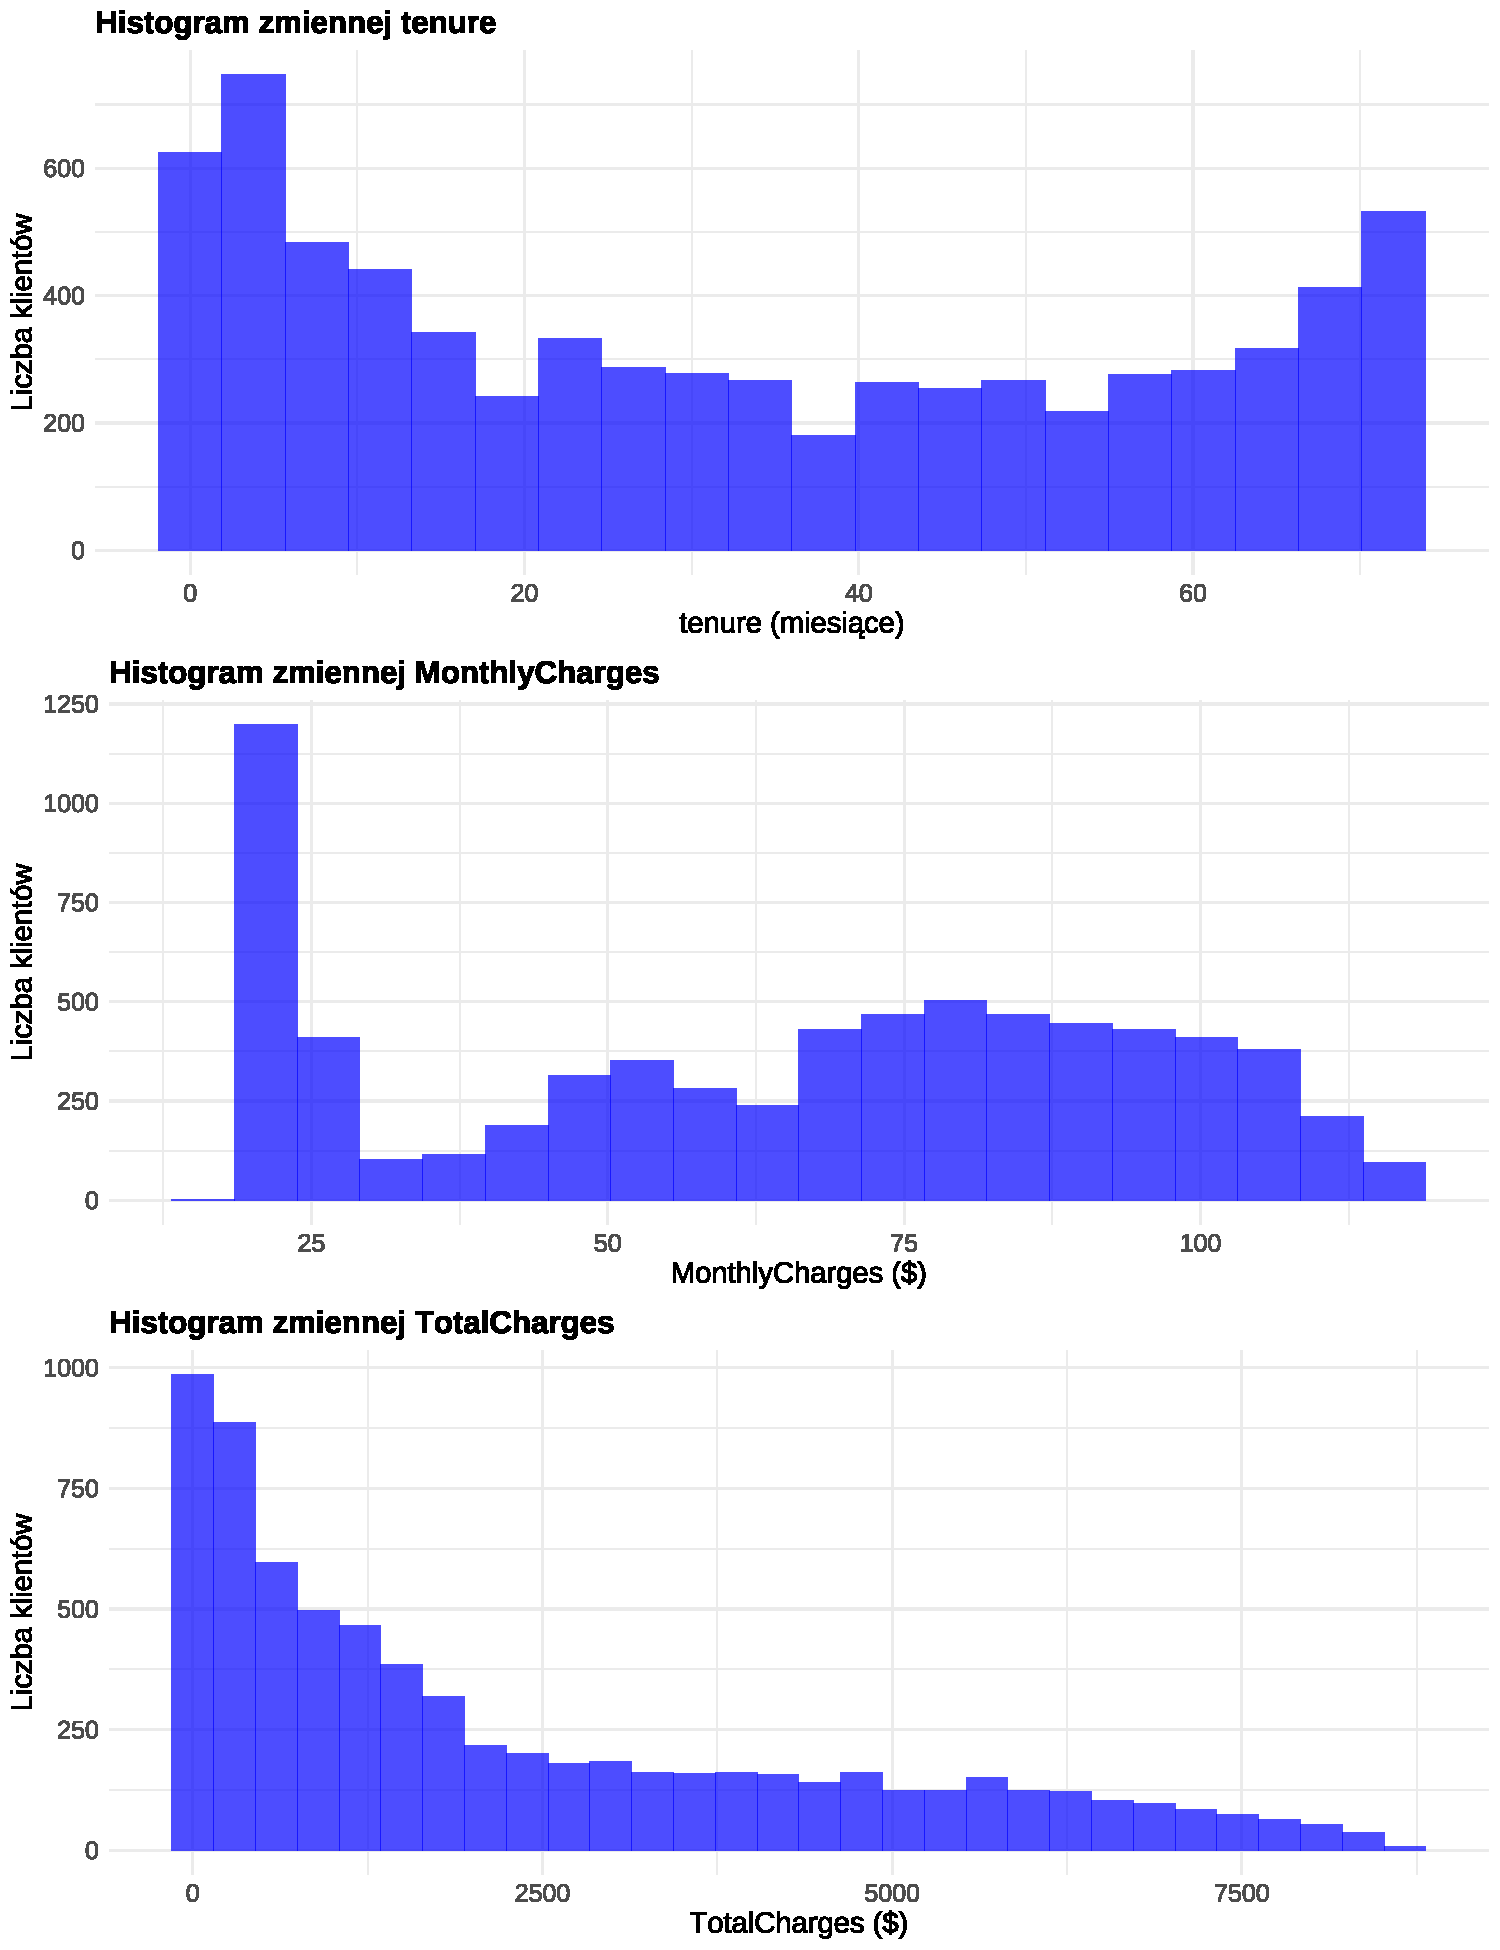
\includegraphics[width=\maxwidth]{figure/histogramy-wszystkie-dane-1} 

}

\caption[Histogramy dla zmiennych ilościowych bez podziału na grupy]{Histogramy dla zmiennych ilościowych bez podziału na grupy}\label{fig:histogramy-wszystkie-dane}
\end{figure}

\end{knitrout}

\subsubsection{Wykresy gęstości}
\begin{knitrout}
\definecolor{shadecolor}{rgb}{0.969, 0.969, 0.969}\color{fgcolor}\begin{figure}[H]

{\centering 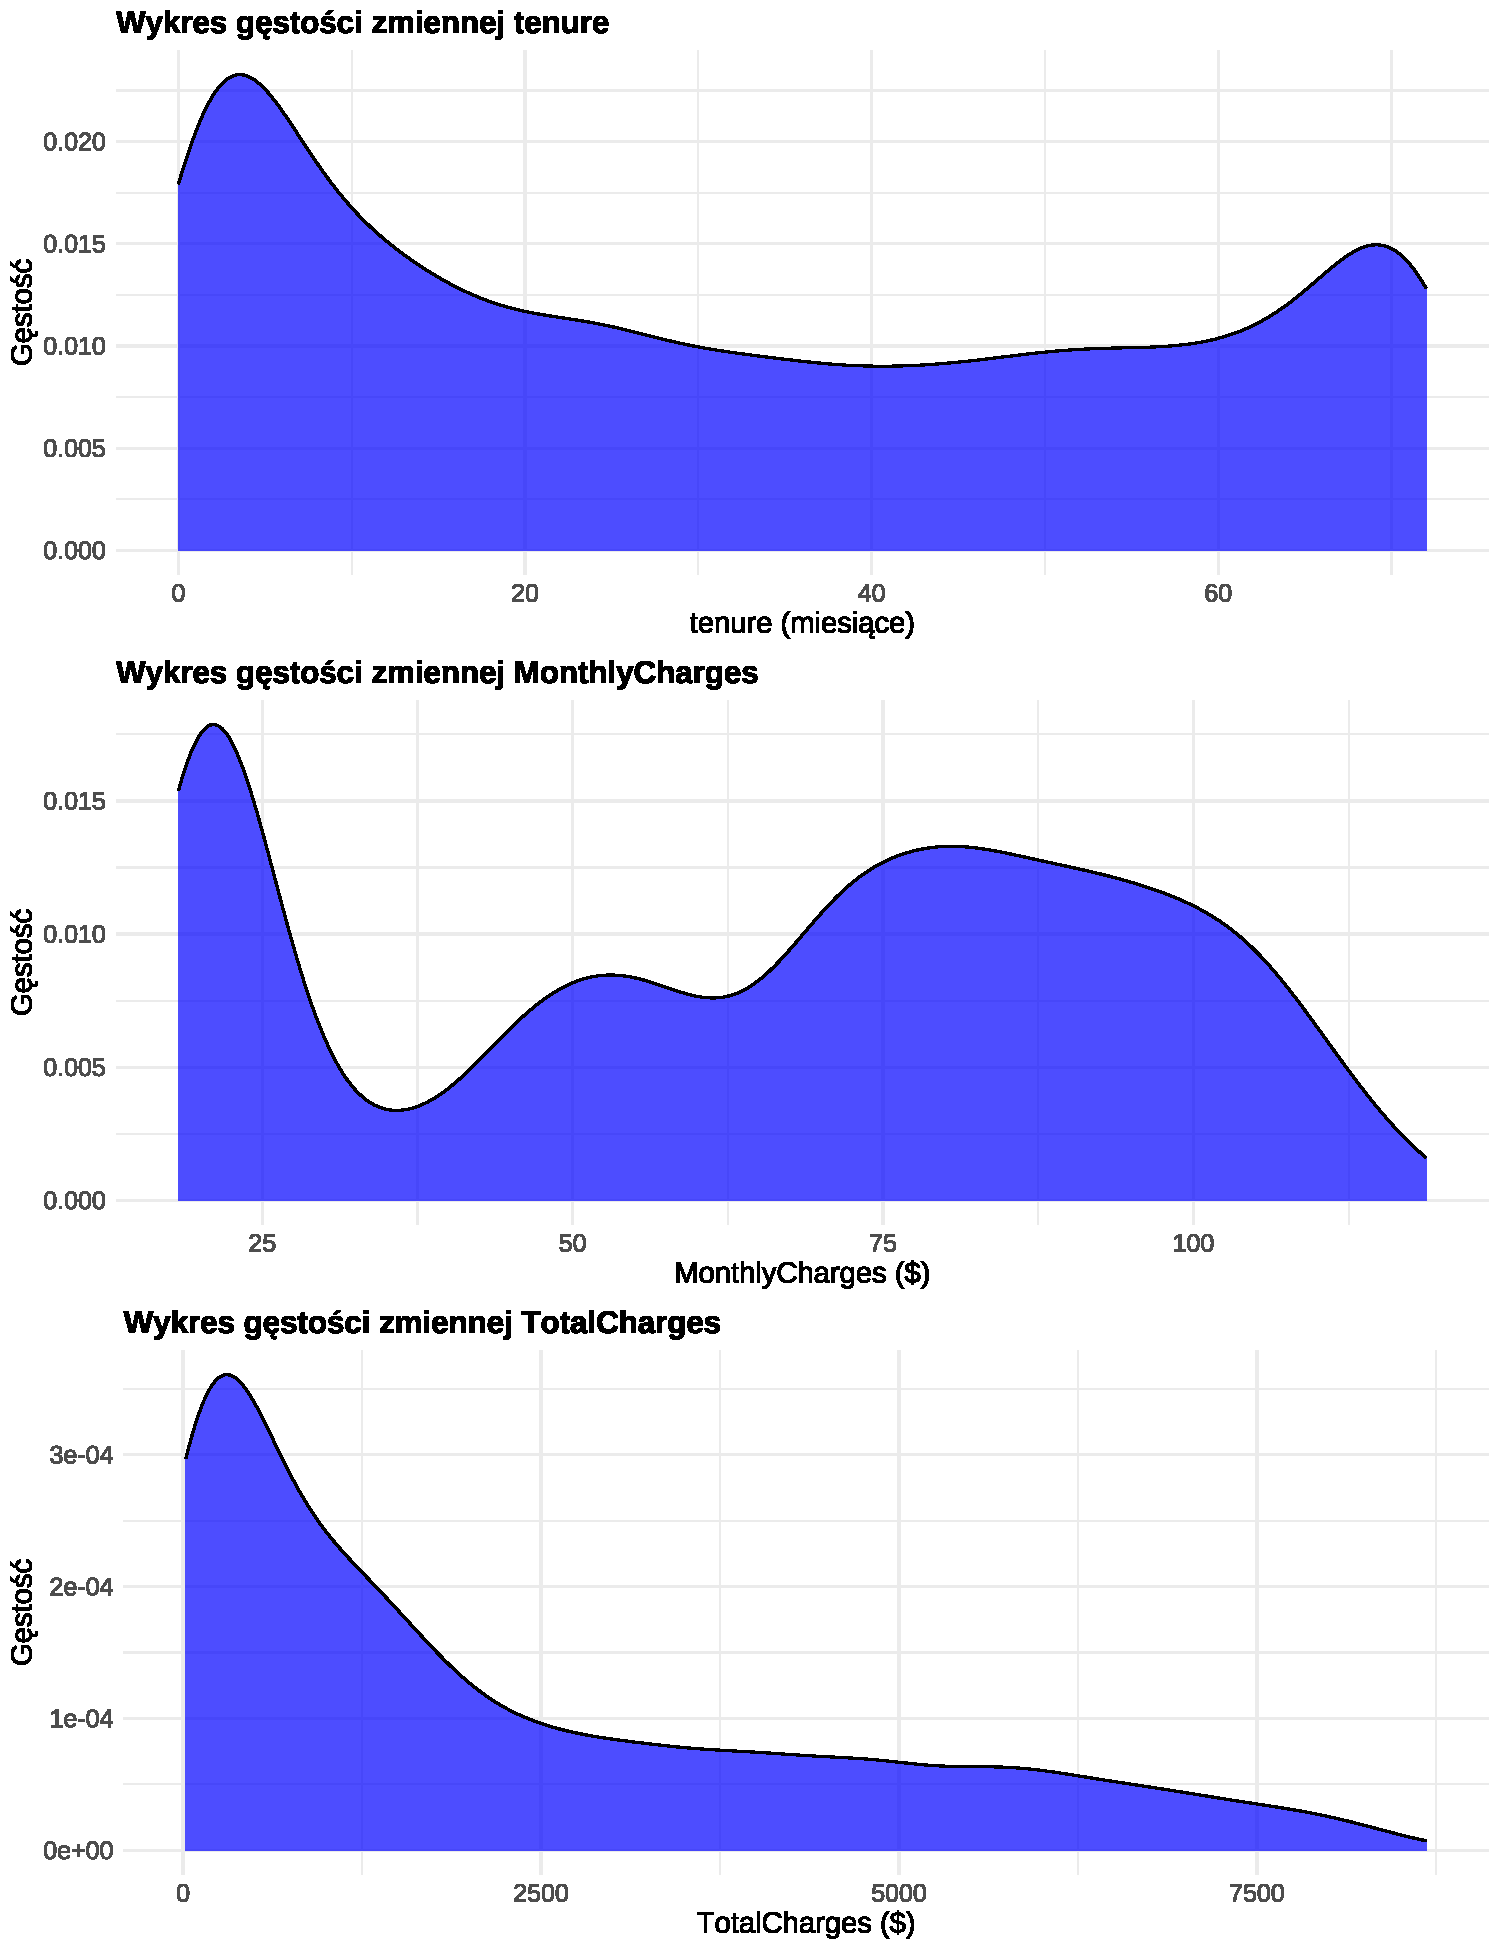
\includegraphics[width=\maxwidth]{figure/gestosc-wszystkie-dane-1} 

}

\caption[Wykresy gęstości dla zmiennych ilościowych bez podziału na grupy]{Wykresy gęstości dla zmiennych ilościowych bez podziału na grupy}\label{fig:gestosc-wszystkie-dane}
\end{figure}

\end{knitrout}


\subsubsection{Wykresy pudełkowe}
\begin{knitrout}
\definecolor{shadecolor}{rgb}{0.969, 0.969, 0.969}\color{fgcolor}\begin{figure}[H]

{\centering 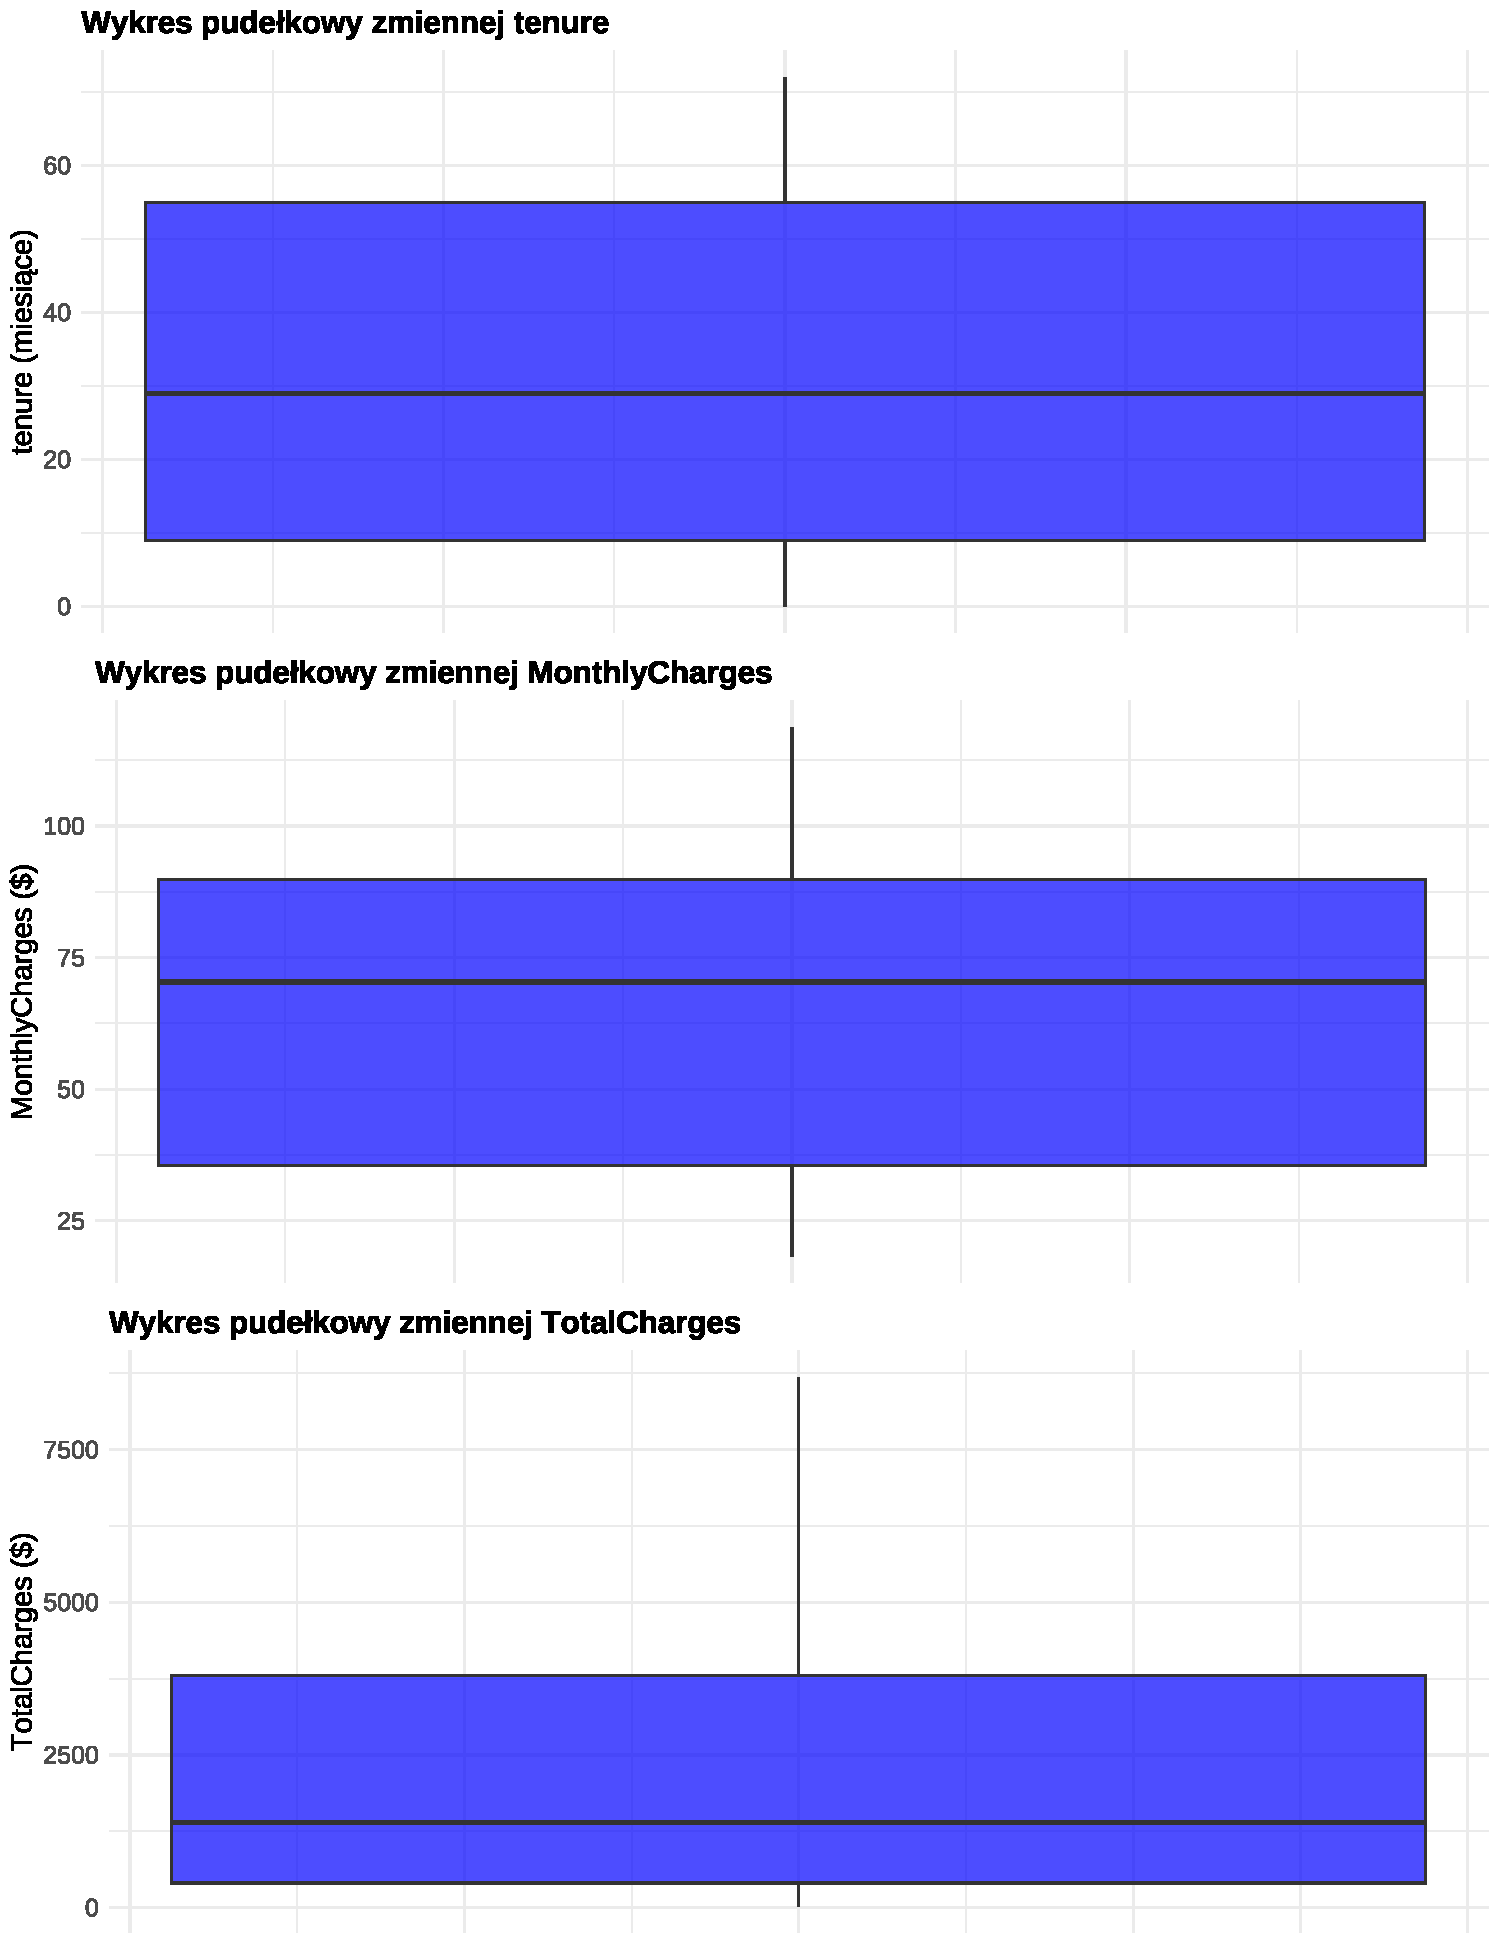
\includegraphics[width=\maxwidth]{figure/boxploty-wszystkie-dane-1} 

}

\caption[Wykresy pudełkowe dla zmiennych ilościowych bez podziału na grupy]{Wykresy pudełkowe dla zmiennych ilościowych bez podziału na grupy}\label{fig:boxploty-wszystkie-dane}
\end{figure}

\end{knitrout}


Analizując dane z tabeli (Tabela \ref{tab:stats_all}), histogramów (Rysunek \ref{fig:histogramy-wszystkie-dane}), wykresów gęstości (Rysunek\ref{fig:gestosc-wszystkie-dane}) i wykresów pudełkowych (Rysunek\ref{fig:boxploty-wszystkie-dane}) można zauważyć, że:

\begin{itemize}
  \item Zmienna \texttt{tenure} ma wartości od 0 do 72 miesięcy, ze średnią 32.4 miesięcy i medianą 29 miesięcy. Rozkład tej zmiennej jest dość równomierny, co sugeruje podobną liczbę klientów z różnym stażem
  
  \item Zmienna \texttt{MonthlyCharges} ma zakres od \$18.25 do \$118.75, ze średnią \$64.76 i medianą \$70.35. Różnica między średnią a medianą sugeruje lekką asymetrię rozkładu. Wykres gęstości pokazuje dwa wyraźne szczyty - pierwszy dla niższych opłat (około 20\$) i drugi dla wyższych (około 80\$)
  
  \item Zmienna \texttt{TotalCharges} ma największe zróżnicowanie, z wartościami od \$18.8 do \$8684.8. Duża różnica między średnią (\$2283.3) a medianą (\$1397.47) wskazuje na wyraźną asymetrię prawostronną rozkładu. Wykres gęstości potwierdza to, pokazując wysoką koncentrację obserwacji w niższych wartościach i długi ogon rozkładu w kierunku wartości wysokich
\end{itemize}



\newpage
\subsubsection{Wykresy rozrzutu}

\begin{knitrout}
\definecolor{shadecolor}{rgb}{0.969, 0.969, 0.969}\color{fgcolor}\begin{figure}[H]

{\centering 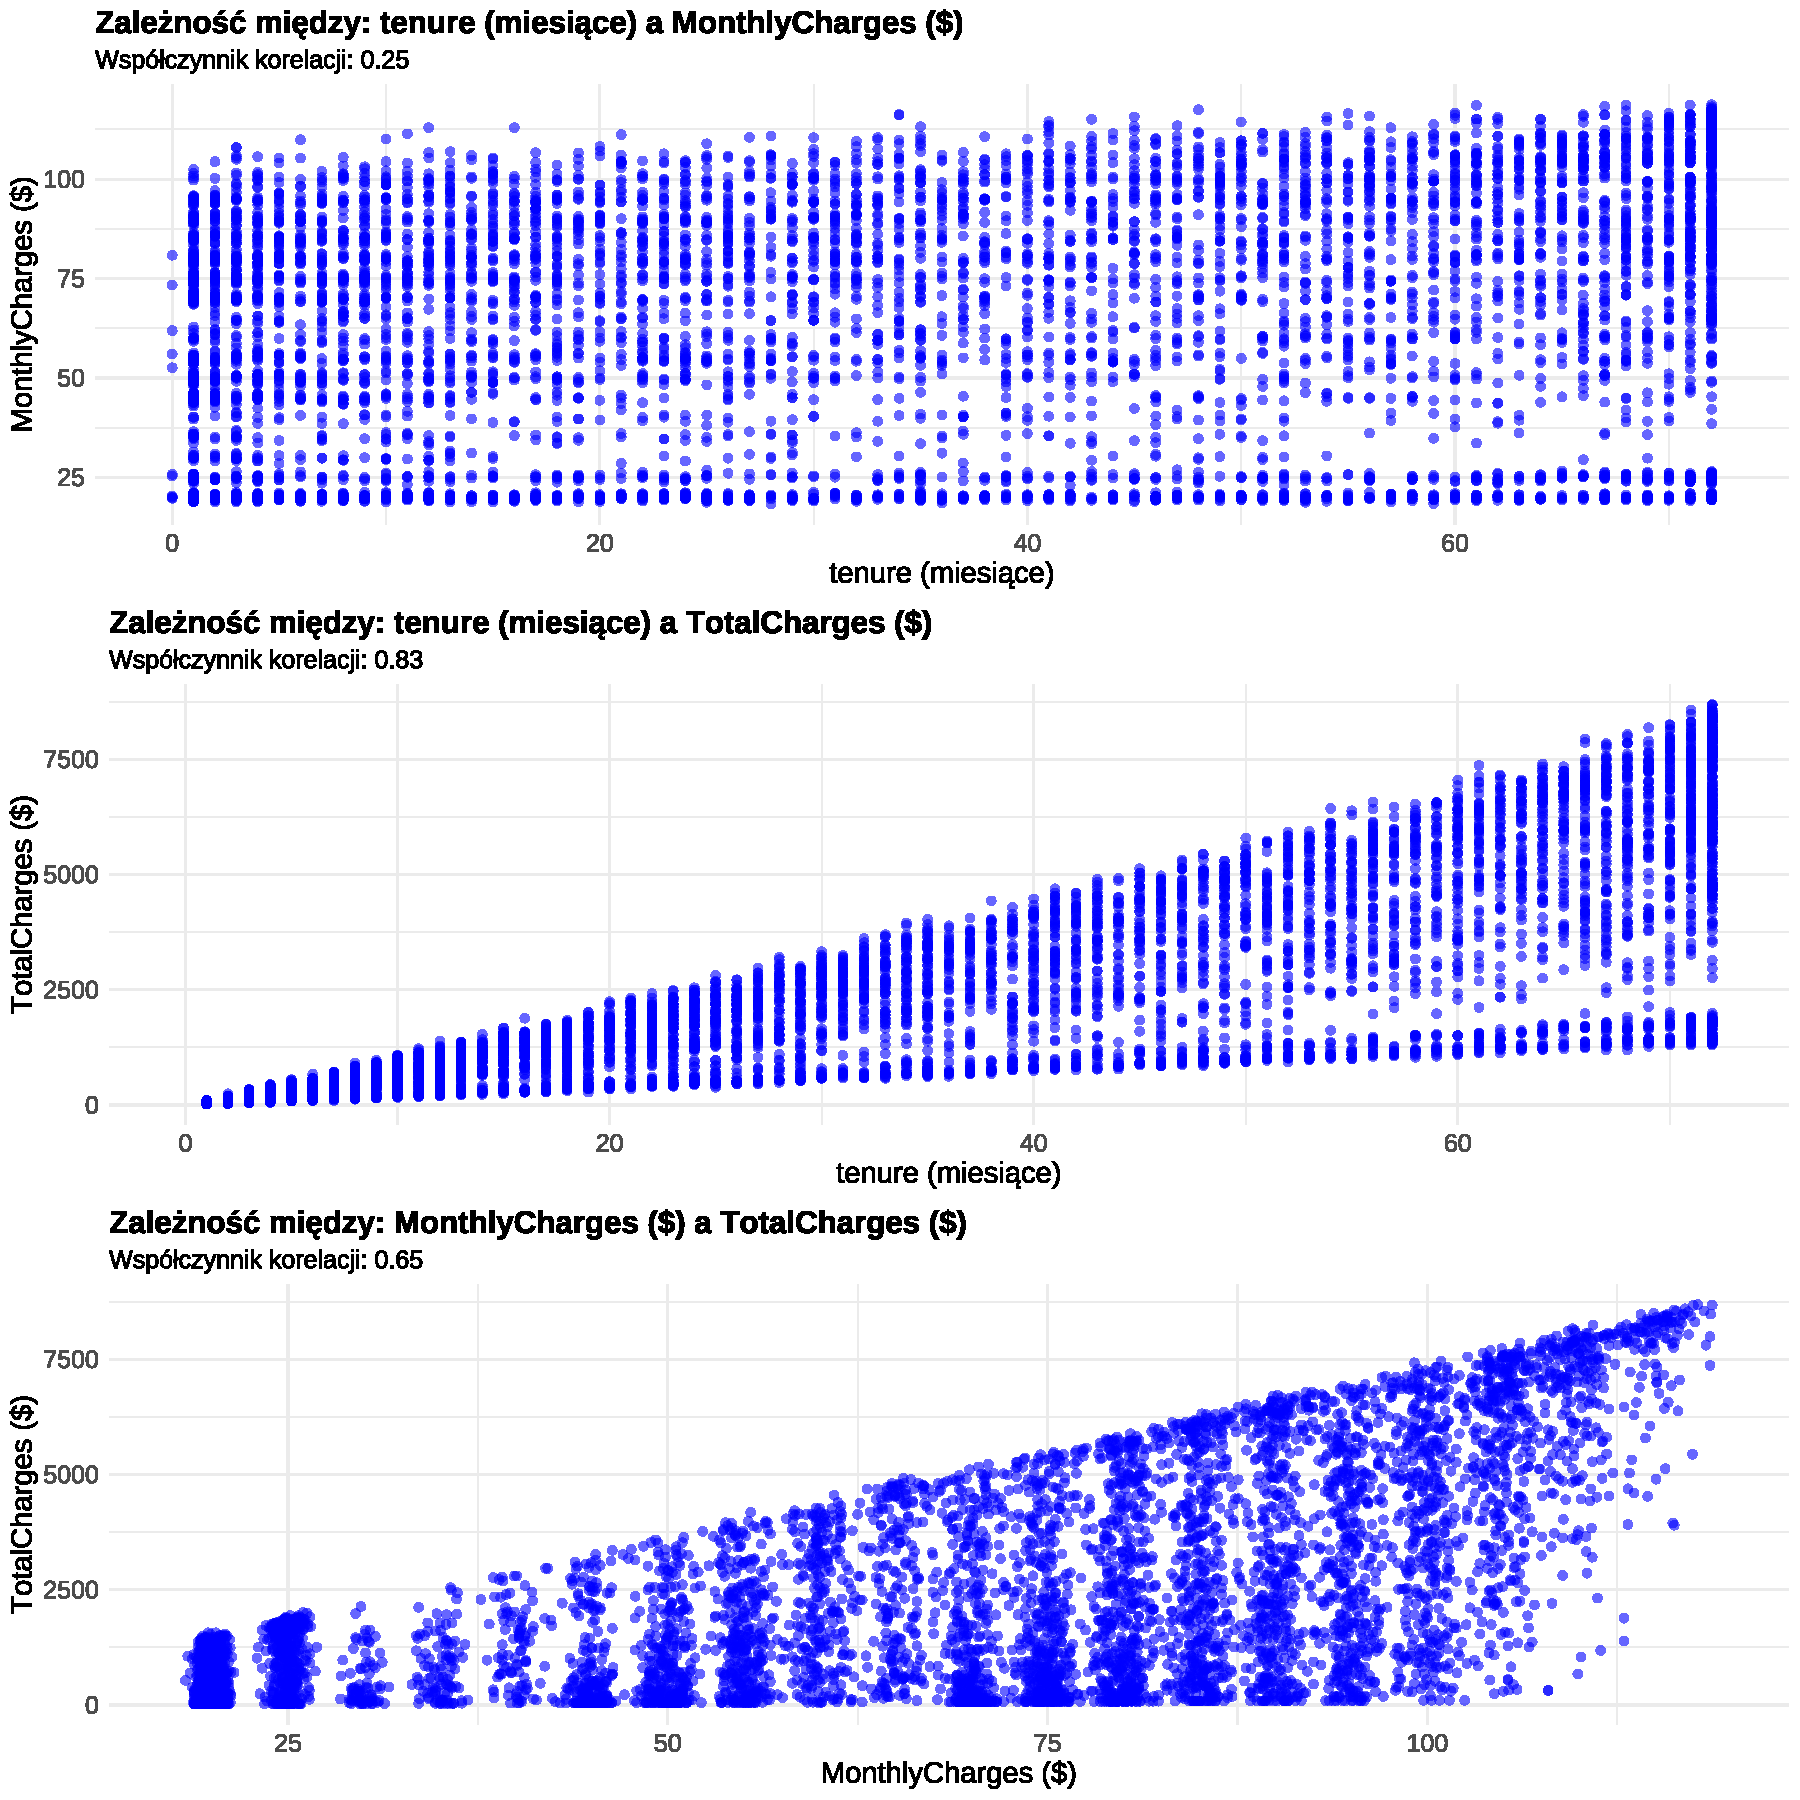
\includegraphics[width=\maxwidth]{figure/scatterploty-wszystkie-dane-1} 

}

\caption[Wykresy rozrzutu dla par zmiennych ilościowych bez podziału na grupy]{Wykresy rozrzutu dla par zmiennych ilościowych bez podziału na grupy}\label{fig:scatterploty-wszystkie-dane}
\end{figure}

\end{knitrout}

\subsubsection{Macierz korelacji}
% latex table generated in R 4.3.2 by xtable 1.8-4 package
% Tue Apr  1 01:14:36 2025
\begin{table}[ht]
\centering
\caption{Macierz korelacji dla zmiennych ilościowych} 
\label{tab:korelacja}
\begin{tabular}{rrrr}
  \hline
 & Okres umowy & MonthlyCharges & TotalCharges \\ 
  \hline
tenure & 1.00 & 0.25 & 0.83 \\ 
  MonthlyCharges & 0.25 & 1.00 & 0.65 \\ 
  TotalCharges & 0.83 & 0.65 & 1.00 \\ 
   \hline
\end{tabular}
\end{table}


\newpage
Na podstawie analizy wykresów rozrzutu (Rysunek \ref{fig:scatterploty-wszystkie-dane}) oraz macierzy korelacji (Tabela \ref{tab:korelacja}), można sformułować następujące wnioski dotyczące zależności między zmiennymi ilościowymi i zmienności poszczególnych cech ilościowych:

\begin{itemize}
  \item Między okresem umowy (\texttt{tenure}) a opłatami całkowitymi (\texttt{TotalCharges}) występuje najsilniejsza zależność liniowa, co potwierdza wysoki współczynnik korelacji wynoszący 0.83. Jest to logiczne, ponieważ im dłużej klient korzysta z usług, tym więcej płaci w sumie. Na wykresie rozrzutu widać wyraźny trend liniowy
    
  \item Między opłatami miesięcznymi (\texttt{MonthlyCharges}) a opłatami całkowitymi (\texttt{TotalCharges}) występuje umiarkowana korelacja (0.65). Związek ten nie jest idealnie liniowy. Na wykresie rozrzutu można zaobserwować duże rozrzut punktów, co potwierdza, że opłaty całkowite zależą nie tylko od wysokości miesięcznych opłat, ale także od okresu umowy
    
  \item Między okresem umowy (\texttt{tenure}) a opłatami miesięcznymi (\texttt{MonthlyCharges}) widoczny jest prawie brak korelacji (0.25), co sugeruje, że wysokość miesięcznych opłat nie zależy od długości relacji klienta z firmą. Wykres rozrzutu dla tej pary zmiennych pokazuje chmurę punktów bez wyraźnego trendu

  \item Największą zmienność wykazują zmienne: 
  \begin{itemize}
      \item \texttt{TotalCharges}, jej punkty są rozproszone w bardzo szerokim zakresie wartości, od bliskich zeru do ponad \$8000
      \item \texttt{tenure}, co widoczne jest w równomiernym rozłożeniu punktów wzdłuż całej osi X (od 0 do ponad 70 miesięcy)
  \end{itemize}
    
\end{itemize}









\newpage
\subsection{Analiza z podziałem na grupy według zmiennej Churn}

\subsubsection{Podstawowe wskaźniki sumaryczne}
% latex table generated in R 4.3.2 by xtable 1.8-4 package
% Tue Apr  1 01:14:36 2025
\begin{table}[ht]
\centering
\caption{Podstawowe statystyki dla klientów, którzy odeszli (Churn = Yes)} 
\label{tab:stats_churn_yes}
\begin{tabular}{rrrr}
  \hline
 & tenure & MonthlyCharges & TotalCharges \\ 
  \hline
Średnia & 17.98 & 74.44 & 1531.80 \\ 
  Mediana & 10.00 & 79.65 & 703.55 \\ 
  Min & 1.00 & 18.85 & 18.85 \\ 
  Max & 72.00 & 118.35 & 8684.80 \\ 
  Q1.25\% & 2.00 & 56.15 & 134.50 \\ 
  Q3.75\% & 29.00 & 94.20 & 2331.30 \\ 
  SD & 19.53 & 24.67 & 1890.82 \\ 
  IQR & 27.00 & 38.05 & 2196.80 \\ 
   \hline
\end{tabular}
\end{table}
% latex table generated in R 4.3.2 by xtable 1.8-4 package
% Tue Apr  1 01:14:36 2025
\begin{table}[ht]
\centering
\caption{Podstawowe statystyki dla klientów lojalnych (Churn = No)} 
\label{tab:stats_churn_no}
\begin{tabular}{rrrr}
  \hline
 & tenure & MonthlyCharges & TotalCharges \\ 
  \hline
Średnia & 37.57 & 61.27 & 2555.34 \\ 
  Mediana & 38.00 & 64.43 & 1683.60 \\ 
  Min & 0.00 & 18.25 & 18.80 \\ 
  Max & 72.00 & 118.75 & 8672.45 \\ 
  Q1.25\% & 15.00 & 25.10 & 577.82 \\ 
  Q3.75\% & 61.00 & 88.40 & 4264.12 \\ 
  SD & 24.11 & 31.09 & 2329.46 \\ 
  IQR & 46.00 & 63.30 & 3686.30 \\ 
   \hline
\end{tabular}
\end{table}


\newpage
\subsubsection{Histogramy}
\begin{knitrout}
\definecolor{shadecolor}{rgb}{0.969, 0.969, 0.969}\color{fgcolor}\begin{figure}[H]

{\centering 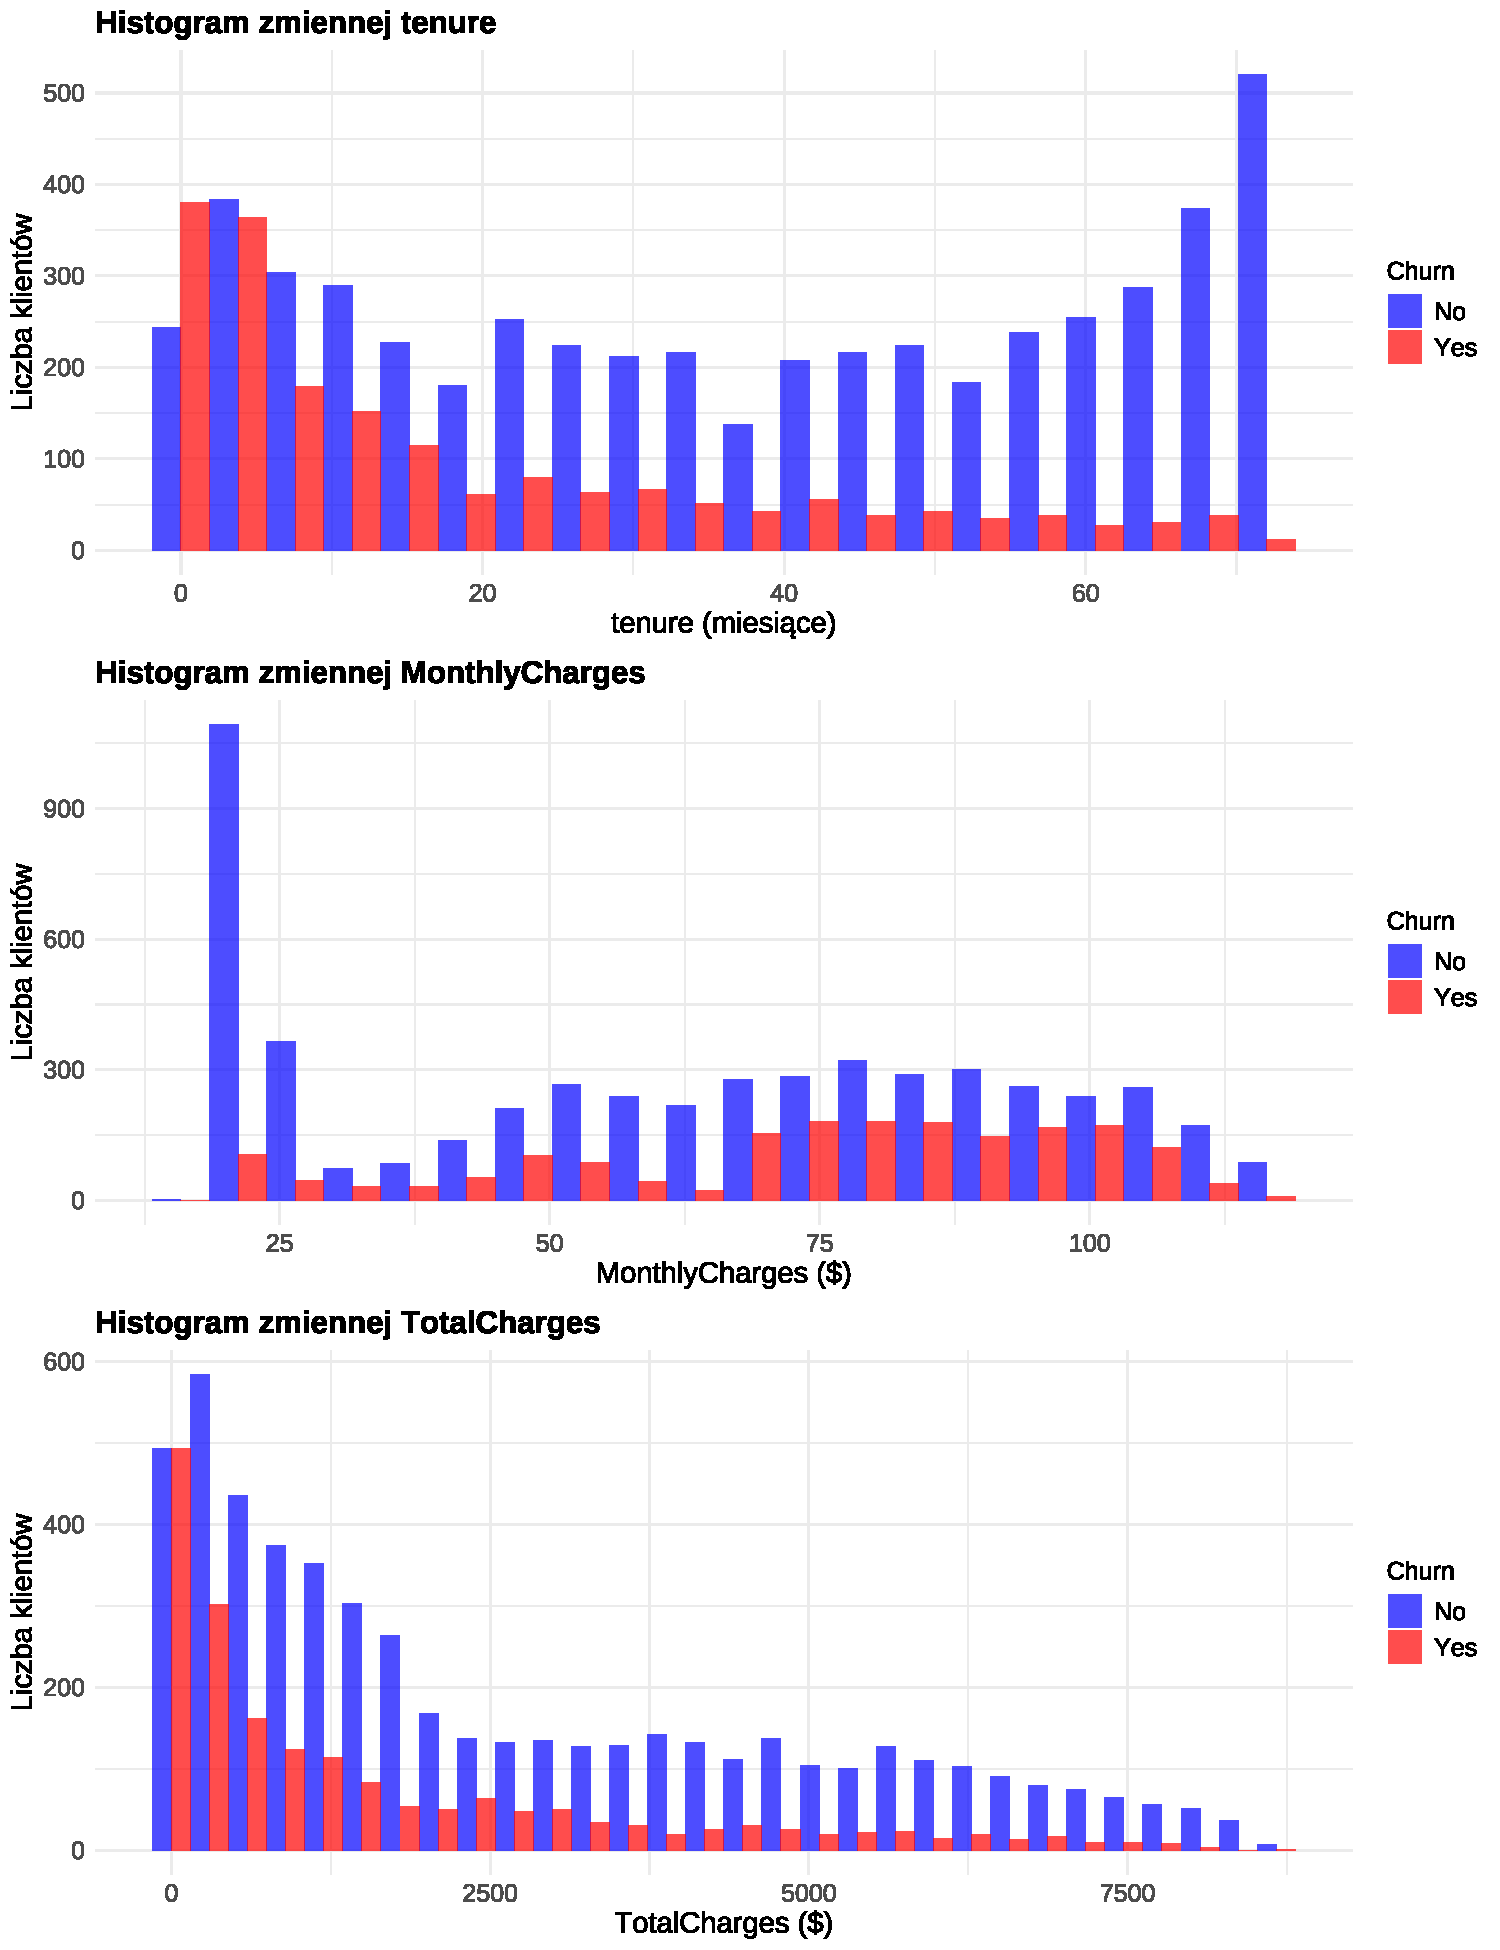
\includegraphics[width=\maxwidth]{figure/histogramy-churn-1} 

}

\caption[Histogramy dla zmiennych ilościowych z podziałem na grupy według zmiennej Churn]{Histogramy dla zmiennych ilościowych z podziałem na grupy według zmiennej Churn}\label{fig:histogramy-churn}
\end{figure}

\end{knitrout}


\newpage
\subsubsection{Wykresy gęstości}
\begin{knitrout}
\definecolor{shadecolor}{rgb}{0.969, 0.969, 0.969}\color{fgcolor}\begin{figure}[H]

{\centering 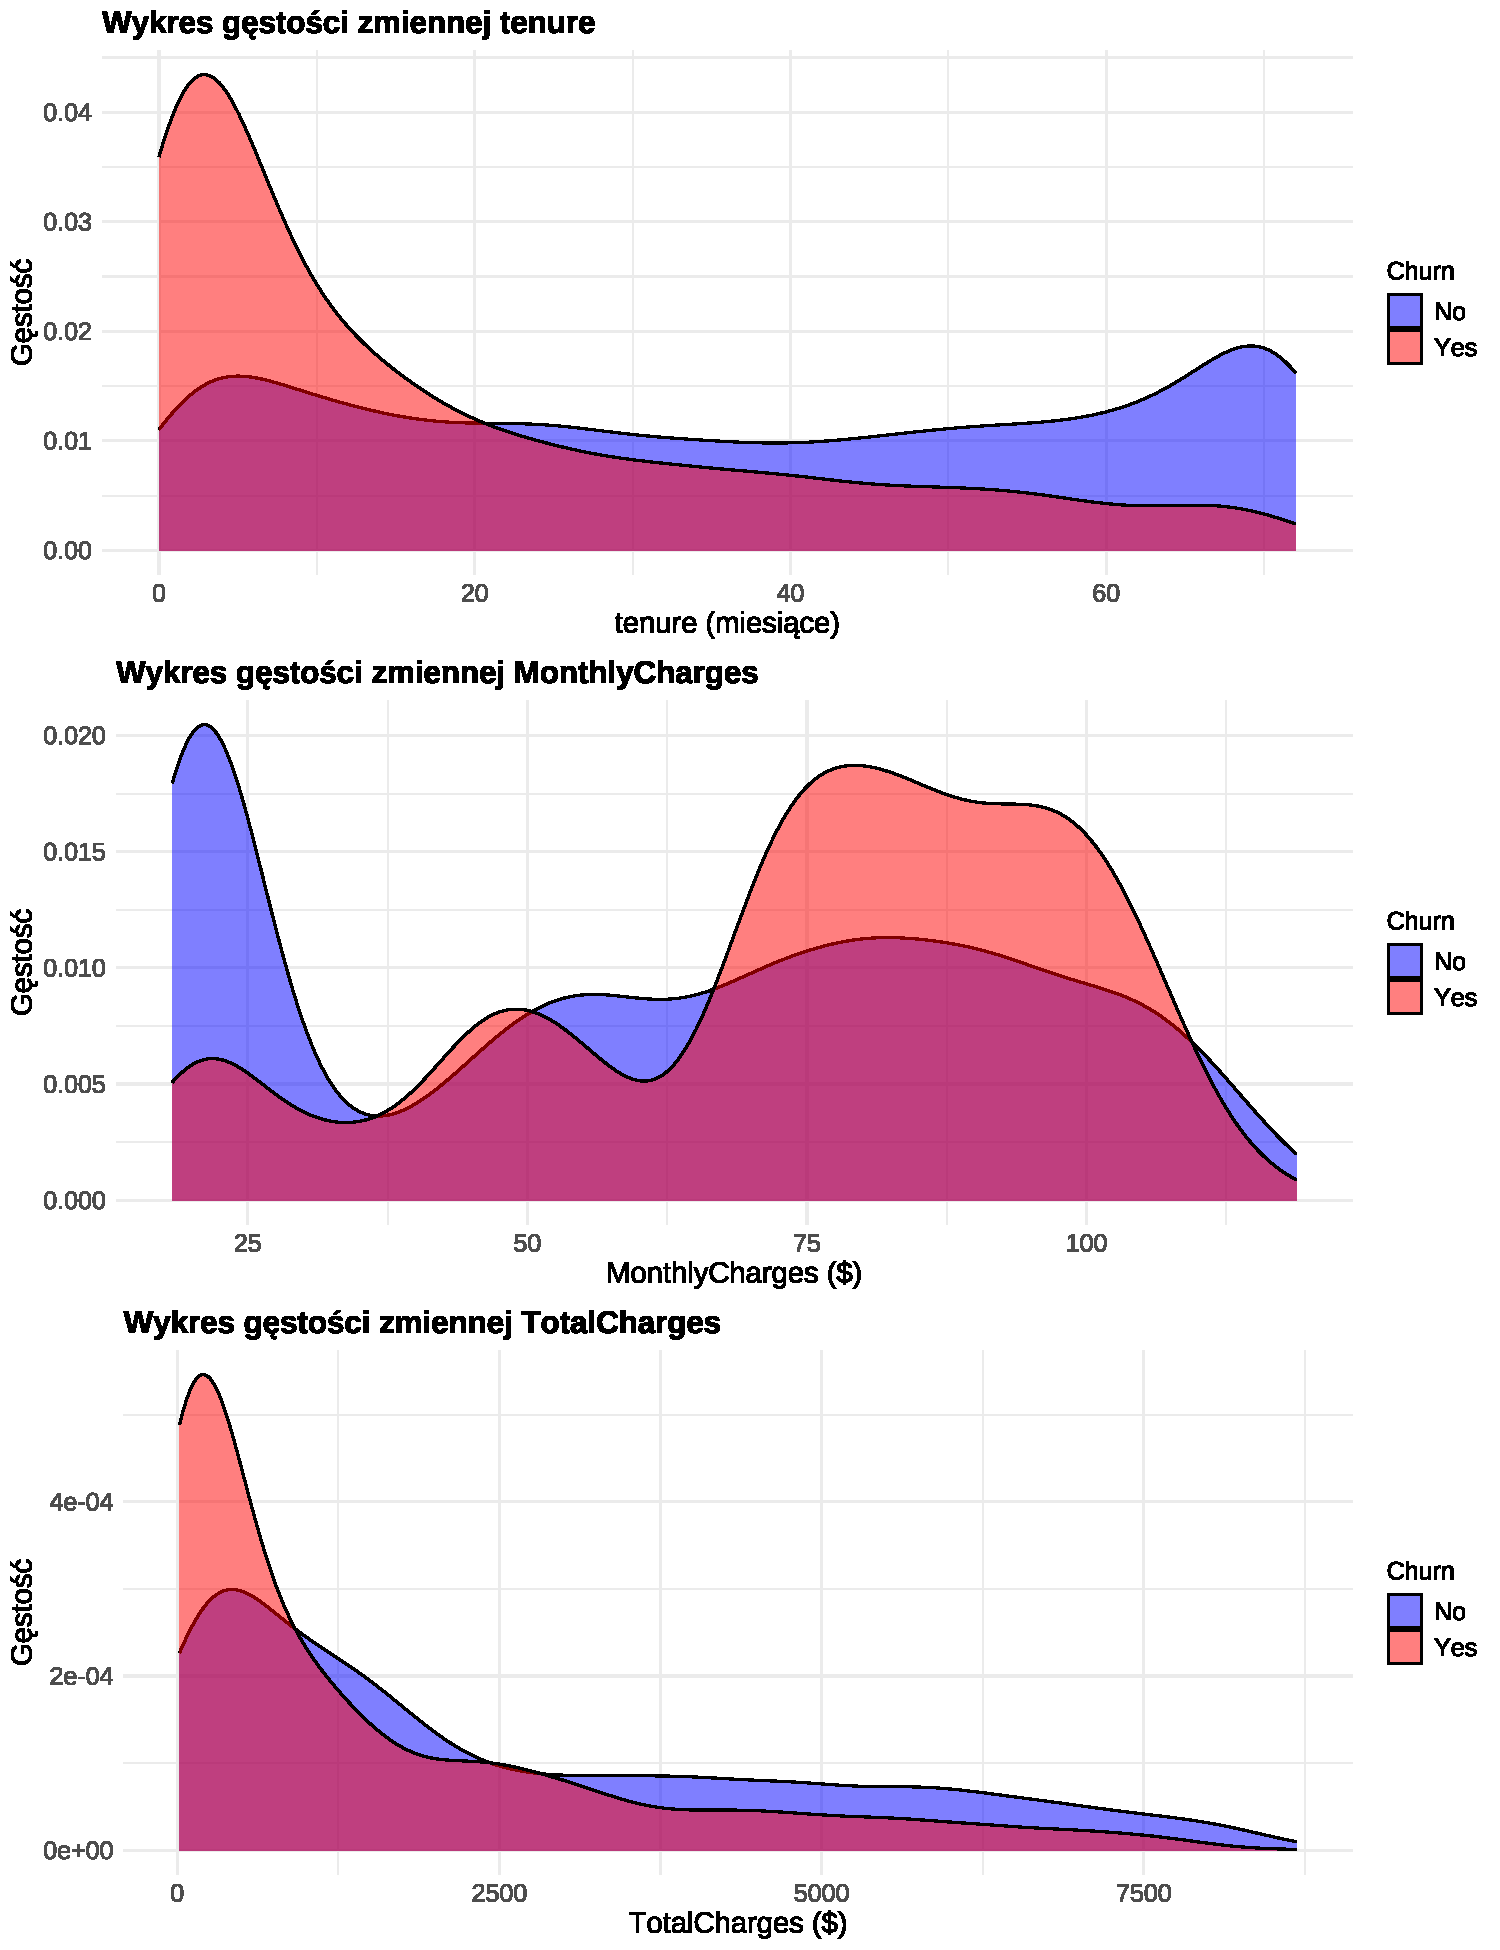
\includegraphics[width=\maxwidth]{figure/gestosc-churn-1} 

}

\caption[Wykresy gęstości dla zmiennych ilościowych z podziałem na grupy według zmiennej Churn]{Wykresy gęstości dla zmiennych ilościowych z podziałem na grupy według zmiennej Churn}\label{fig:gestosc-churn}
\end{figure}

\end{knitrout}


\subsubsection{Wykresy pudełkowe}
\begin{knitrout}
\definecolor{shadecolor}{rgb}{0.969, 0.969, 0.969}\color{fgcolor}\begin{figure}[H]

{\centering 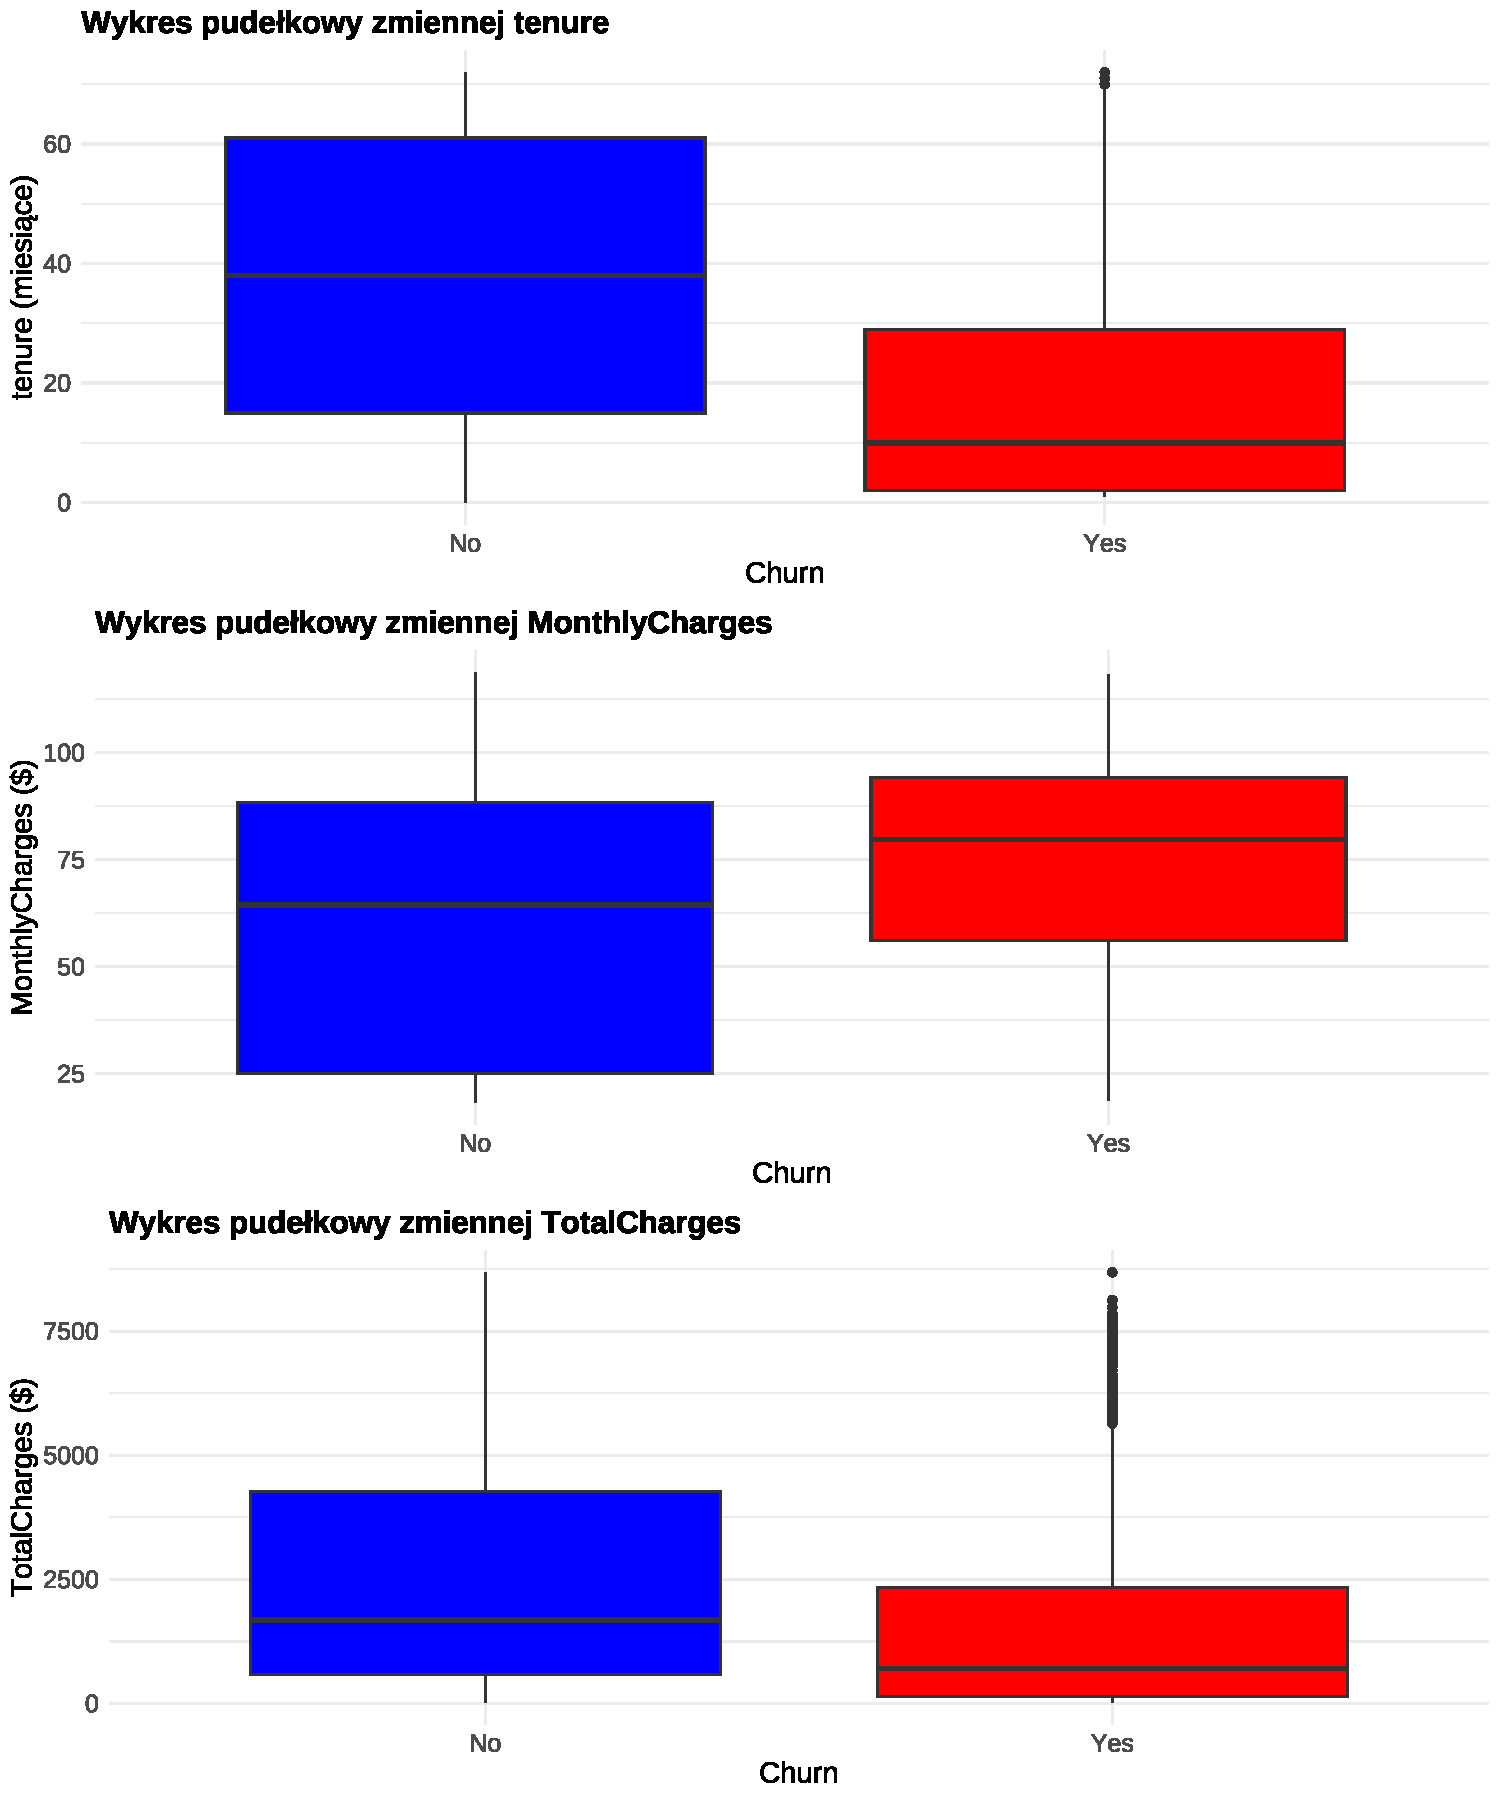
\includegraphics[width=\maxwidth]{figure/boxploty-churn-1} 

}

\caption[Wykresy pudełkowe dla zmiennych ilościowych z podziałem na grupy według zmiennej Churn]{Wykresy pudełkowe dla zmiennych ilościowych z podziałem na grupy według zmiennej Churn}\label{fig:boxploty-churn}
\end{figure}

\end{knitrout}

\newpage
Analizując dane z tabel (Tabela \ref{tab:stats_churn_yes} i \ref{tab:stats_churn_no}), histogramów (Rysunek \ref{fig:histogramy-churn}), wykresów gęstości (Rysunek \ref{fig:gestosc-churn}) oraz wykresów pudełkowych (Rysunek \ref{fig:boxploty-churn}) dla grup wydzielonych według zmiennej Churn, można zauważyć, że:

\begin{itemize}
  \item Zmienna \texttt{tenure} wykazuje znaczące różnice między grupami:
  \begin{itemize}
    \item Dla klientów, którzy odeszli, średnia wynosi jedynie 18 miesięcy, podczas gdy dla lojalnych klientów - 37.6 miesięcy
    \item Mediana dla klientów odchodzących to 10 miesięcy, w porównaniu do 38 miesięcy dla klientów lojalnych
    \item Wykres gęstości pokazuje, że większość rezygnacji następuje w początkowym okresie umowy - rozkład dla grupy Churn=Yes jest silnie prawoskośny
  \end{itemize}
  
  \item Zmienna \texttt{MonthlyCharges} również wykazuje istotne różnice:
  \begin{itemize}
    \item Klienci, którzy odeszli, płacili średnio \$74.44 miesięcznie wobec \$61.27 dla klientów lojalnych
    \item Wykresy pudełkowe ujawniają, że mediana i kwartyle dla klientów rezygnujących są wyraźnie przesunięte w kierunku wyższych wartości
    \item Wykres gęstości dla klientów, którzy odeszli, ma większe zagęszczenie w obszarze wysokich opłat miesięcznych (70-100\$)
  \end{itemize}
  
  \item Zmienna \texttt{TotalCharges} pokazuje:
  \begin{itemize}
    \item Klienci rezygnujący mają niższe średnie opłaty całkowite (\$1531.8) niż klienci lojalni (\$2555.34) (co jest naturalną konsekwencją krótszego okresu umów klientów rezygnujących)
    \item Wykresy pokazują, że dla klientów rezygnujących rozkład jest silnie skoncentrowany w obszarze niskich wartości
  \end{itemize}
\end{itemize}


\newpage
\subsubsection{Wykresy rozrzutu}
\begin{knitrout}
\definecolor{shadecolor}{rgb}{0.969, 0.969, 0.969}\color{fgcolor}\begin{figure}[H]

{\centering 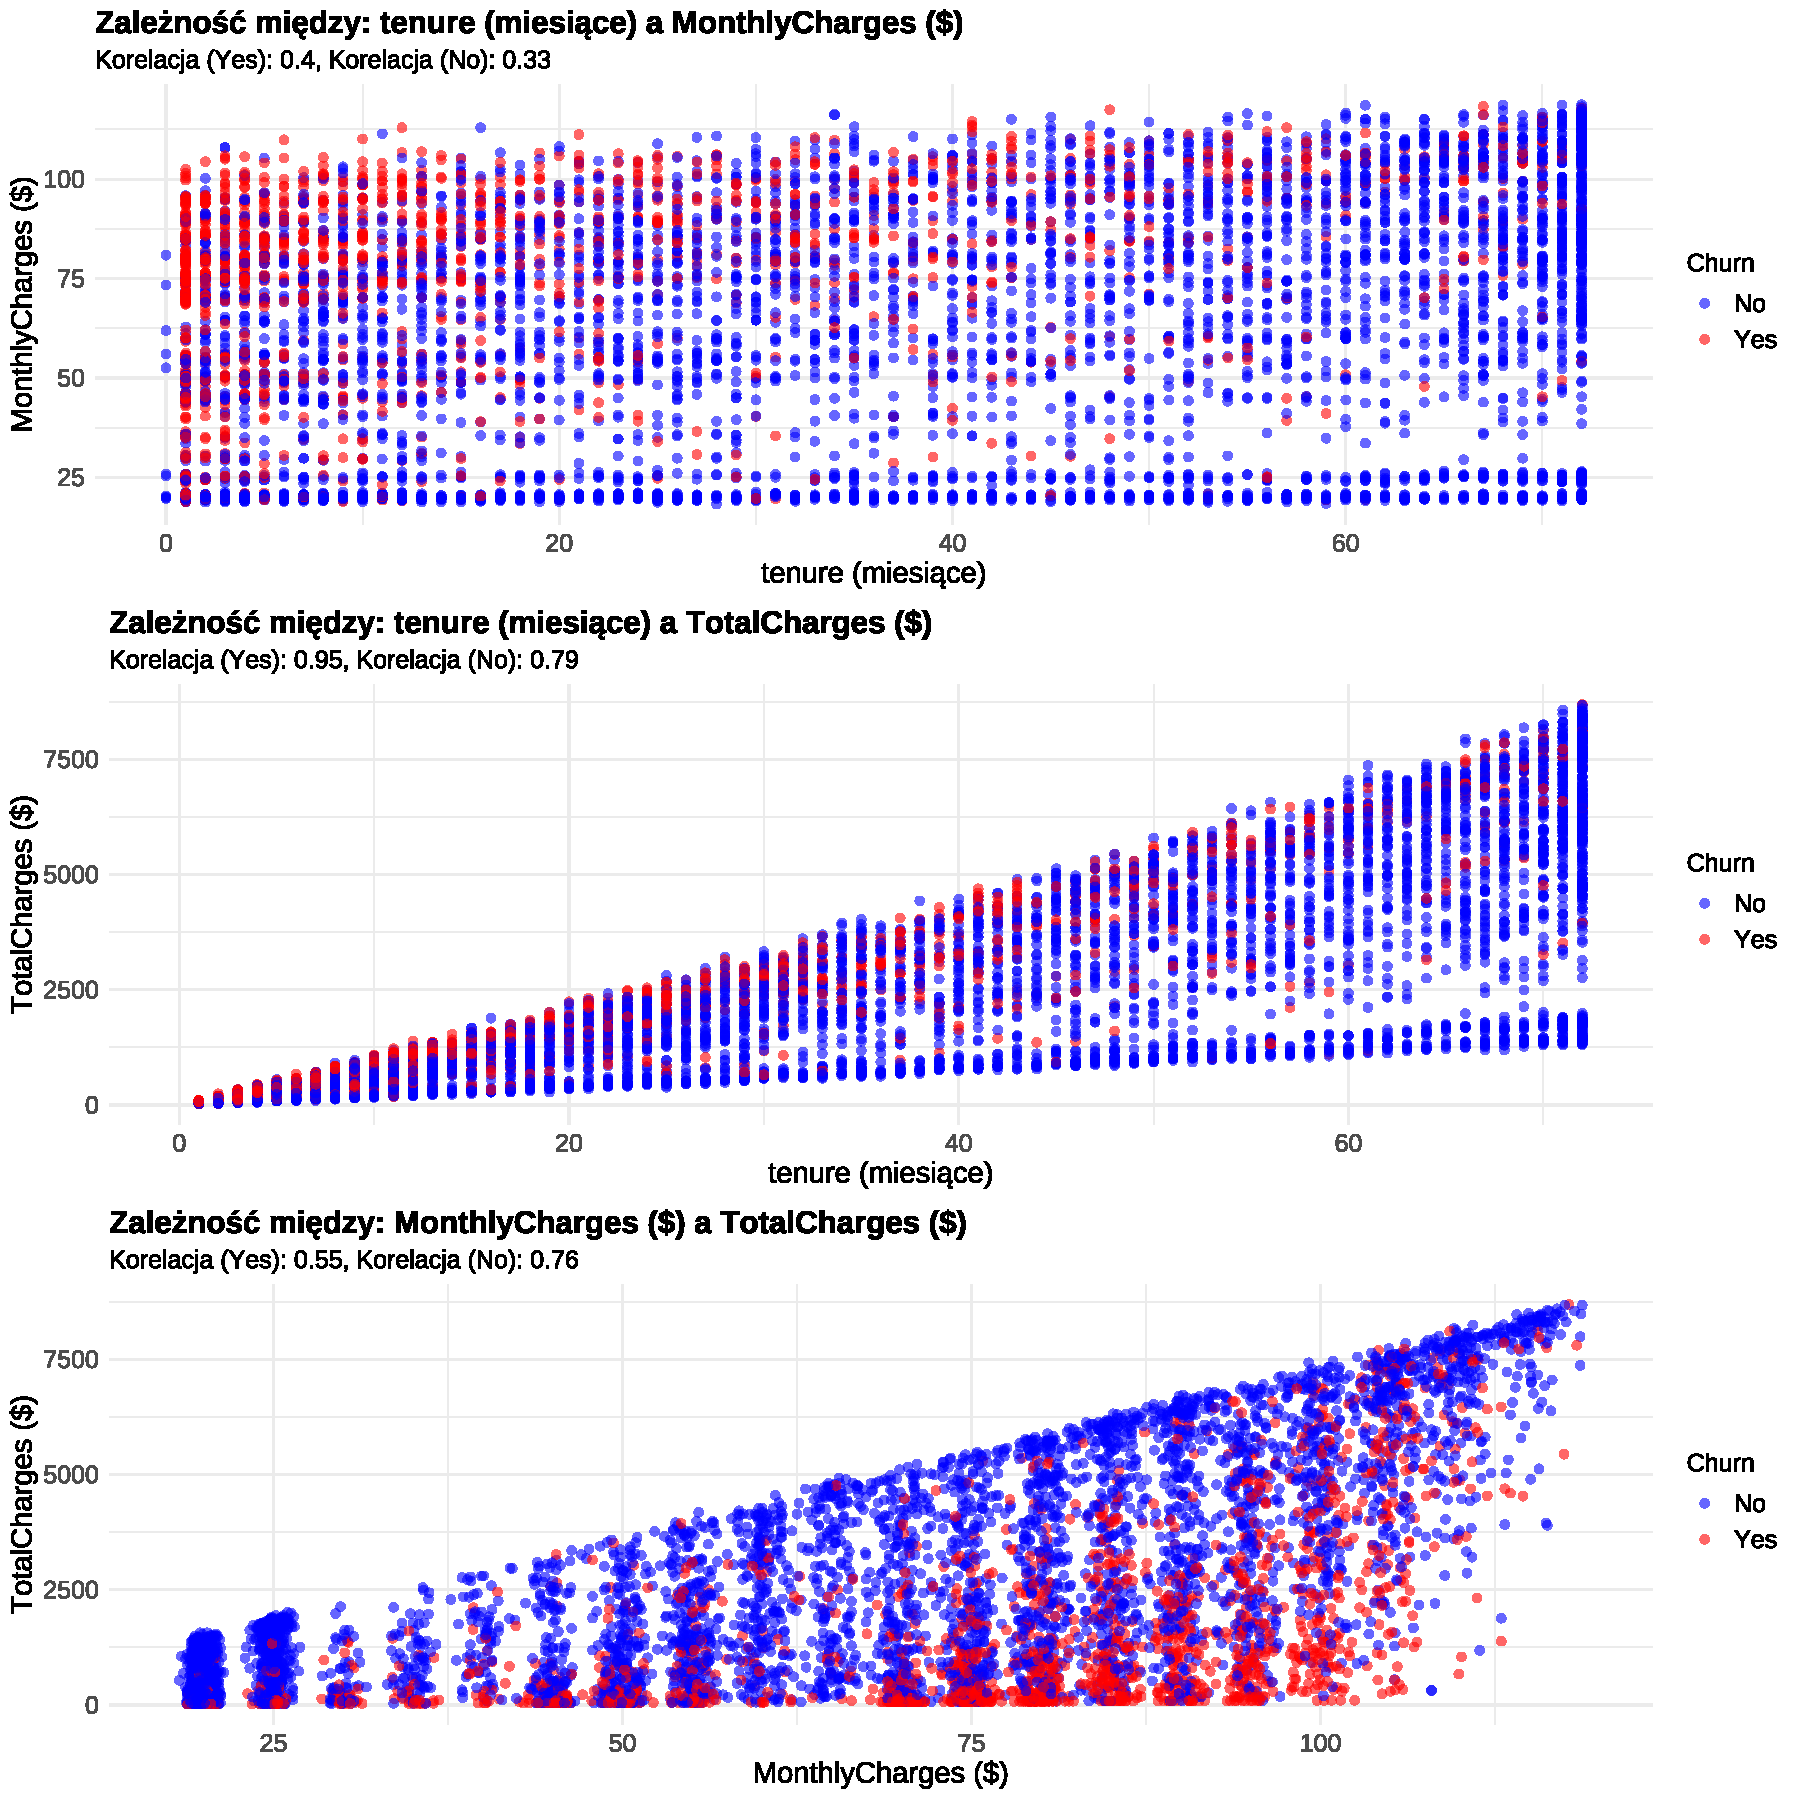
\includegraphics[width=\maxwidth]{figure/scatterploty-churn-1} 

}

\caption[Wykresy rozrzutu dla par zmiennych ilościowych z podziałem na grupy według zmiennej Churn]{Wykresy rozrzutu dla par zmiennych ilościowych z podziałem na grupy według zmiennej Churn}\label{fig:scatterploty-churn}
\end{figure}

\end{knitrout}


\subsubsection{Macierze korelacji}
% latex table generated in R 4.3.2 by xtable 1.8-4 package
% Tue Apr  1 01:14:38 2025
\begin{table}[ht]
\centering
\caption{Macierz korelacji dla klientów, którzy odeszli (Churn = Yes)} 
\label{tab:korelacja_yes}
\begin{tabular}{rrrr}
  \hline
 & tenure & MonthlyCharges & TotalCharges \\ 
  \hline
tenure & 1.00 & 0.40 & 0.95 \\ 
  MonthlyCharges & 0.40 & 1.00 & 0.55 \\ 
  TotalCharges & 0.95 & 0.55 & 1.00 \\ 
   \hline
\end{tabular}
\end{table}
% latex table generated in R 4.3.2 by xtable 1.8-4 package
% Tue Apr  1 01:14:38 2025
\begin{table}[ht]
\centering
\caption{Macierz korelacji dla klientów lojalnych (Churn = No)} 
\label{tab:korelacja_no}
\begin{tabular}{rrrr}
  \hline
 & tenure & MonthlyCharges & TotalCharges \\ 
  \hline
tenure & 1.00 & 0.33 & 0.79 \\ 
  MonthlyCharges & 0.33 & 1.00 & 0.76 \\ 
  TotalCharges & 0.79 & 0.76 & 1.00 \\ 
   \hline
\end{tabular}
\end{table}



Na podstawie analizy wykresów rozrzutu (Rysunek \ref{fig:scatterploty-churn}) oraz macierzy korelacji (Tabela \ref{tab:korelacja_yes} i \ref{tab:korelacja_no}), można sformułować następujące wnioski dotyczące zależności między zmiennymi ilościowymi w obu grupach klientów:

\begin{itemize}
  \item Korelacja między \texttt{tenure} a \texttt{TotalCharges} jest silna w obu grupach:
  \begin{itemize}
    \item Dla klientów, którzy odeszli, współczynnik korelacji wynosi 0.95
    \item Dla klientów lojalnych współczynnik korelacji wynosi 0.79
    \item Na wykresie rozrzutu widać, że punkty reprezentujące klientów, którzy odeszli, są skoncentrowane w lewym dolnym rogu (krótki okres, niskie opłaty całkowite)
  \end{itemize}
    
  \item Korelacja między \texttt{MonthlyCharges} a \texttt{TotalCharges} wykazuje różnice między grupami:
  \begin{itemize}
    \item Dla klientów, którzy odeszli, korelacja jest słabsza (0.55) niż dla klientów lojalnych (0.76)
    \item Niższa korelacja w grupie klientów rezygnujących może wynikać z ich krótkiego okresu umowy, który ogranicza wpływ opłat miesięcznych na wartość całkowitą
  \end{itemize}
    
  \item Relacja między \texttt{tenure} a \texttt{MonthlyCharges} ujawnia niewielkie różnice między grupami:
  \begin{itemize}
    \item Dla klientów, którzy odeszli, występuje umiarkowana dodatnia korelacja (0.4)
    \item Dla klientów lojalnych korelacja jest również dodatnia, choć nieco słabsza (0.33)
    \item Sugeruje to, że szczególnie w grupie klientów rezygnujących, dłuższy okres umowy jest powiązany z wyższymi opłatami miesięcznymi - być może ci klienci decydują się na rozwiązanie umowy właśnie z powodu rosnących kosztów
  \end{itemize}

Zmiennymi najlepiej różnicującymi obie grupy są:
  \begin{itemize}
    \item \texttt{tenure} - bardzo wyraźna separacja grup na wykresach, największa różnica średnich i median
    \item \texttt{MonthlyCharges} - widoczna różnica w rozkładach, klienci rezygnujący płacą więcej miesięcznie
  \end{itemize}
    
\end{itemize}





\newpage
\section{Analiza zmiennych jakościowych}
W dalszej analizie skupimy się na zmiennych, które wykazują największe zróżnicowanie w danych oraz potencjalnie najsilniejszy związek ze zmienną objaśnianą \texttt{Churn}. Zmienne takie jak \texttt{SeniorCitizen}, \texttt{Partner}, \texttt{Dependents}, \texttt{Contract}, \texttt{PaperlessBilling} oraz \texttt{TechSupport} będą głównym przedmiotem analizy, podczas gdy zmienne o dużej liczbie brakujących danych lub też zmienne nic nie wnoszące do analizy zostaną pominięte, aby uniknąć wprowadzania szumów do analizy.

\subsection{Analiza dla zbioru bez podziału na grupy}

\subsubsection{Tabele częstości}
% latex table generated in R 4.3.2 by xtable 1.8-4 package
% Tue Apr  1 01:14:38 2025
\begin{table}[ht]
\centering
\caption{Tabela częstości dla zmiennej: SeniorCitizen} 
\label{tab:czest_SeniorCitizen}
\begin{tabular}{lrr}
  \hline
Kategoria & Liczebność & Procent \\ 
  \hline
0 & 5901 & 83.79 \\ 
  1 & 1142 & 16.21 \\ 
   \hline
\end{tabular}
\end{table}
% latex table generated in R 4.3.2 by xtable 1.8-4 package
% Tue Apr  1 01:14:38 2025
\begin{table}[ht]
\centering
\caption{Tabela częstości dla zmiennej: Partner} 
\label{tab:czest_Partner}
\begin{tabular}{lrr}
  \hline
Kategoria & Liczebność & Procent \\ 
  \hline
No & 3641 & 51.70 \\ 
  Yes & 3402 & 48.30 \\ 
   \hline
\end{tabular}
\end{table}
% latex table generated in R 4.3.2 by xtable 1.8-4 package
% Tue Apr  1 01:14:38 2025
\begin{table}[ht]
\centering
\caption{Tabela częstości dla zmiennej: Dependents} 
\label{tab:czest_Dependents}
\begin{tabular}{lrr}
  \hline
Kategoria & Liczebność & Procent \\ 
  \hline
No & 4933 & 70.04 \\ 
  Yes & 2110 & 29.96 \\ 
   \hline
\end{tabular}
\end{table}
% latex table generated in R 4.3.2 by xtable 1.8-4 package
% Tue Apr  1 01:14:38 2025
\begin{table}[ht]
\centering
\caption{Tabela częstości dla zmiennej: Contract} 
\label{tab:czest_Contract}
\begin{tabular}{lrr}
  \hline
Kategoria & Liczebność & Procent \\ 
  \hline
Month-to-month & 3875 & 55.02 \\ 
  One year & 1473 & 20.91 \\ 
  Two year & 1695 & 24.07 \\ 
   \hline
\end{tabular}
\end{table}
% latex table generated in R 4.3.2 by xtable 1.8-4 package
% Tue Apr  1 01:14:38 2025
\begin{table}[ht]
\centering
\caption{Tabela częstości dla zmiennej: PaperlessBilling} 
\label{tab:czest_PaperlessBilling}
\begin{tabular}{lrr}
  \hline
Kategoria & Liczebność & Procent \\ 
  \hline
No & 2872 & 40.78 \\ 
  Yes & 4171 & 59.22 \\ 
   \hline
\end{tabular}
\end{table}
% latex table generated in R 4.3.2 by xtable 1.8-4 package
% Tue Apr  1 01:14:38 2025
\begin{table}[ht]
\centering
\caption{Tabela częstości dla zmiennej: TechSupport} 
\label{tab:czest_TechSupport}
\begin{tabular}{lrr}
  \hline
Kategoria & Liczebność & Procent \\ 
  \hline
No & 3473 & 49.31 \\ 
  No internet service & 1526 & 21.67 \\ 
  Yes & 2044 & 29.02 \\ 
   \hline
\end{tabular}
\end{table}



\clearpage
\subsubsection{Wykresy słupkowe}
\begin{knitrout}
\definecolor{shadecolor}{rgb}{0.969, 0.969, 0.969}\color{fgcolor}\begin{figure}[H]

{\centering 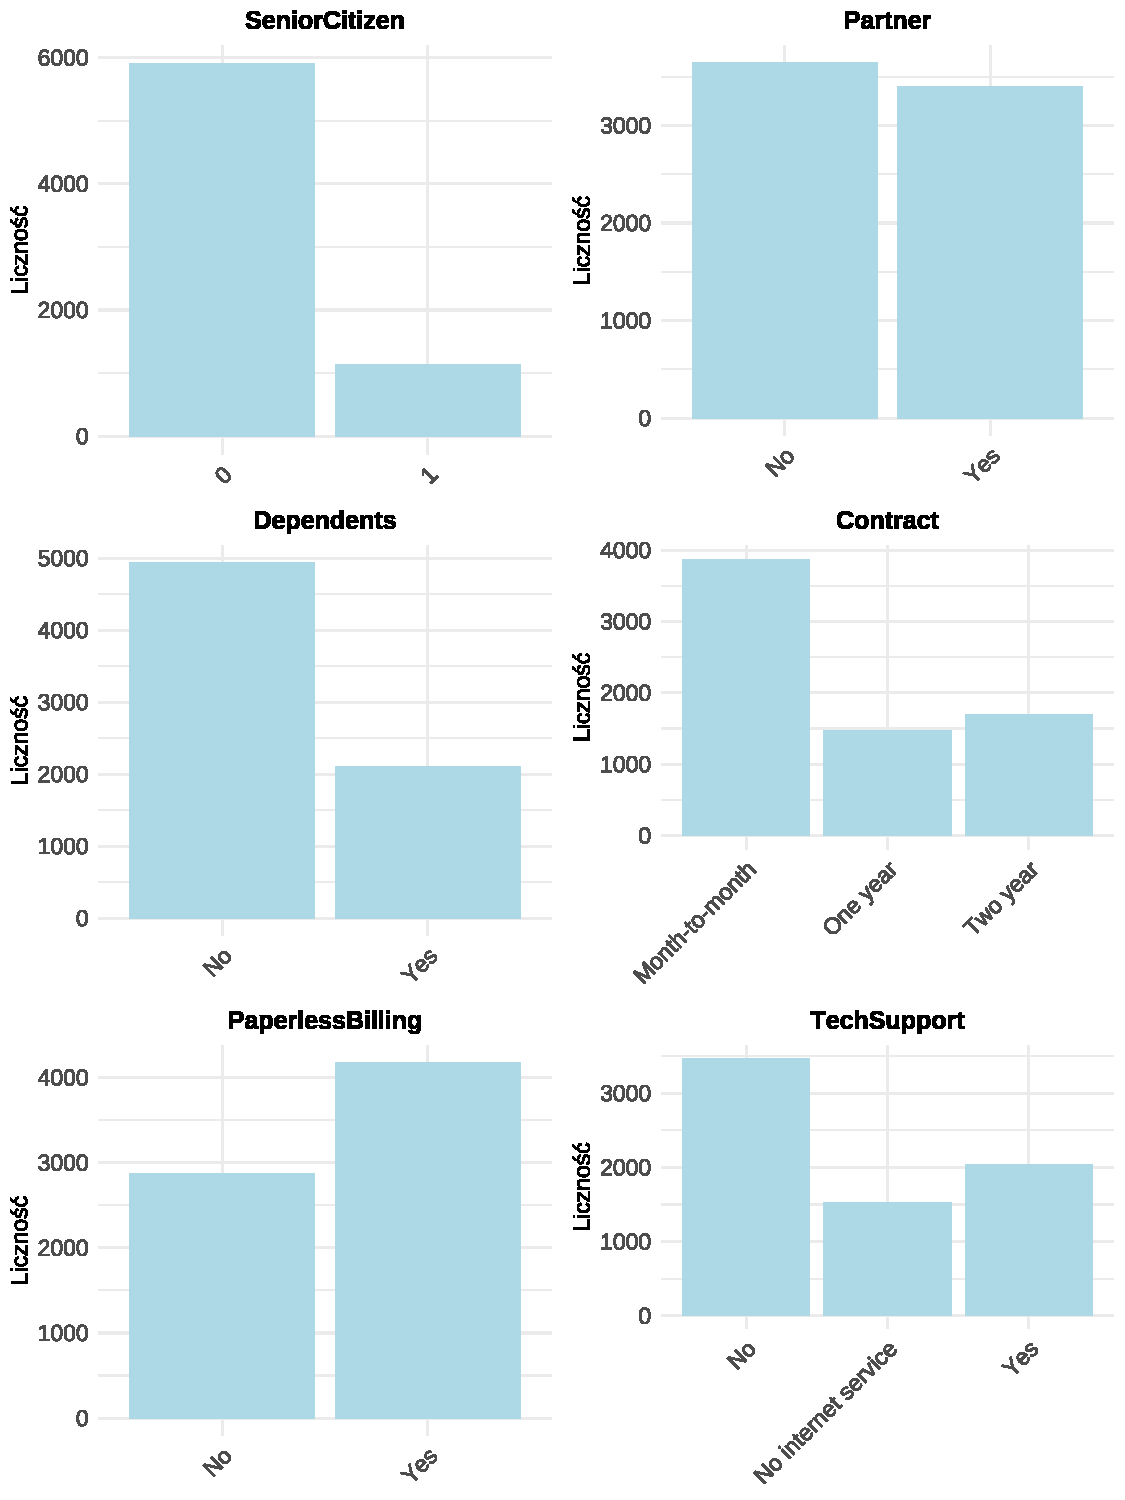
\includegraphics[width=0.85\textwidth]{figure/wykresy-slupkowe-1} 

}

\caption{\label{fig:wykresy-slupkowe} Wykresy słupkowe przedstawiające rozkład częstości najważniejszych zmiennych jakościowych}\label{fig:wykresy-slupkowe}
\end{figure}

\end{knitrout}

\newpage
Jak przedstawiono na wykresach słupkowych (Rysunek \ref{fig:wykresy-slupkowe}), zmienne jakościowe w zbiorze danych charakteryzują się różnymi rozkładami. Szczególnie istotna jest zmienna \texttt{Contract} (rodzaj umowy), gdzie dominują umowy miesięczne, oraz zmienna \texttt{SeniorCitizen}, pokazująca że zdecydowana większość klientów to osoby młodsze. Zmienne \texttt{Partner} i \texttt{Dependents} wskazują, że większość klientów nie posiada partnerów ani osób zależnych. Zmienna \texttt{TechSupport} pokazuje, że znaczna część klientów nie korzysta z usług wsparcia technicznego, co może mieć istotne znaczenie w kontekście ich satysfakcji z usług.



\subsection{Analiza dla zbioru z podziałem na grupy według zmiennej Churn}

\subsubsection{Tabele częstości}
% latex table generated in R 4.3.2 by xtable 1.8-4 package
% Tue Apr  1 01:14:38 2025
\begin{table}[ht]
\centering
\caption{Tabela częstości dla zmiennej SeniorCitizen z podziałem na Churn} 
\label{tab:churn_SeniorCitizen}
\begin{tabular}{lrrr}
  \hline
Kategoria & Liczba\_klientow & Liczba\_odchodzacych & Procent\_odchodzacych \\ 
  \hline
0 & 5901.00 & 1393 & 23.61 \\ 
  1 & 1142.00 & 476 & 41.68 \\ 
   \hline
\end{tabular}
\end{table}
% latex table generated in R 4.3.2 by xtable 1.8-4 package
% Tue Apr  1 01:14:38 2025
\begin{table}[ht]
\centering
\caption{Tabela częstości dla zmiennej Partner z podziałem na Churn} 
\label{tab:churn_Partner}
\begin{tabular}{lrrr}
  \hline
Kategoria & Liczba\_klientow & Liczba\_odchodzacych & Procent\_odchodzacych \\ 
  \hline
No & 3641.00 & 1200 & 32.96 \\ 
  Yes & 3402.00 & 669 & 19.66 \\ 
   \hline
\end{tabular}
\end{table}
% latex table generated in R 4.3.2 by xtable 1.8-4 package
% Tue Apr  1 01:14:38 2025
\begin{table}[ht]
\centering
\caption{Tabela częstości dla zmiennej Dependents z podziałem na Churn} 
\label{tab:churn_Dependents}
\begin{tabular}{lrrr}
  \hline
Kategoria & Liczba\_klientow & Liczba\_odchodzacych & Procent\_odchodzacych \\ 
  \hline
No & 4933.00 & 1543 & 31.28 \\ 
  Yes & 2110.00 & 326 & 15.45 \\ 
   \hline
\end{tabular}
\end{table}
% latex table generated in R 4.3.2 by xtable 1.8-4 package
% Tue Apr  1 01:14:38 2025
\begin{table}[ht]
\centering
\caption{Tabela częstości dla zmiennej Contract z podziałem na Churn} 
\label{tab:churn_Contract}
\begin{tabular}{lrrr}
  \hline
Kategoria & Liczba\_klientow & Liczba\_odchodzacych & Procent\_odchodzacych \\ 
  \hline
Month-to-month & 3875.00 & 1655 & 42.71 \\ 
  One year & 1473.00 & 166 & 11.27 \\ 
  Two year & 1695.00 &  48 & 2.83 \\ 
   \hline
\end{tabular}
\end{table}
% latex table generated in R 4.3.2 by xtable 1.8-4 package
% Tue Apr  1 01:14:38 2025
\begin{table}[ht]
\centering
\caption{Tabela częstości dla zmiennej PaperlessBilling z podziałem na Churn} 
\label{tab:churn_PaperlessBilling}
\begin{tabular}{lrrr}
  \hline
Kategoria & Liczba\_klientow & Liczba\_odchodzacych & Procent\_odchodzacych \\ 
  \hline
No & 2872.00 & 469 & 16.33 \\ 
  Yes & 4171.00 & 1400 & 33.57 \\ 
   \hline
\end{tabular}
\end{table}
% latex table generated in R 4.3.2 by xtable 1.8-4 package
% Tue Apr  1 01:14:38 2025
\begin{table}[ht]
\centering
\caption{Tabela częstości dla zmiennej TechSupport z podziałem na Churn} 
\label{tab:churn_TechSupport}
\begin{tabular}{lrrr}
  \hline
Kategoria & Liczba\_klientow & Liczba\_odchodzacych & Procent\_odchodzacych \\ 
  \hline
No & 3473.00 & 1446 & 41.64 \\ 
  No internet service & 1526.00 & 113 & 7.40 \\ 
  Yes & 2044.00 & 310 & 15.17 \\ 
   \hline
\end{tabular}
\end{table}

\clearpage

\subsubsection{Wykresy słupkowe}
\begin{knitrout}
\definecolor{shadecolor}{rgb}{0.969, 0.969, 0.969}\color{fgcolor}\begin{figure}[H]

{\centering 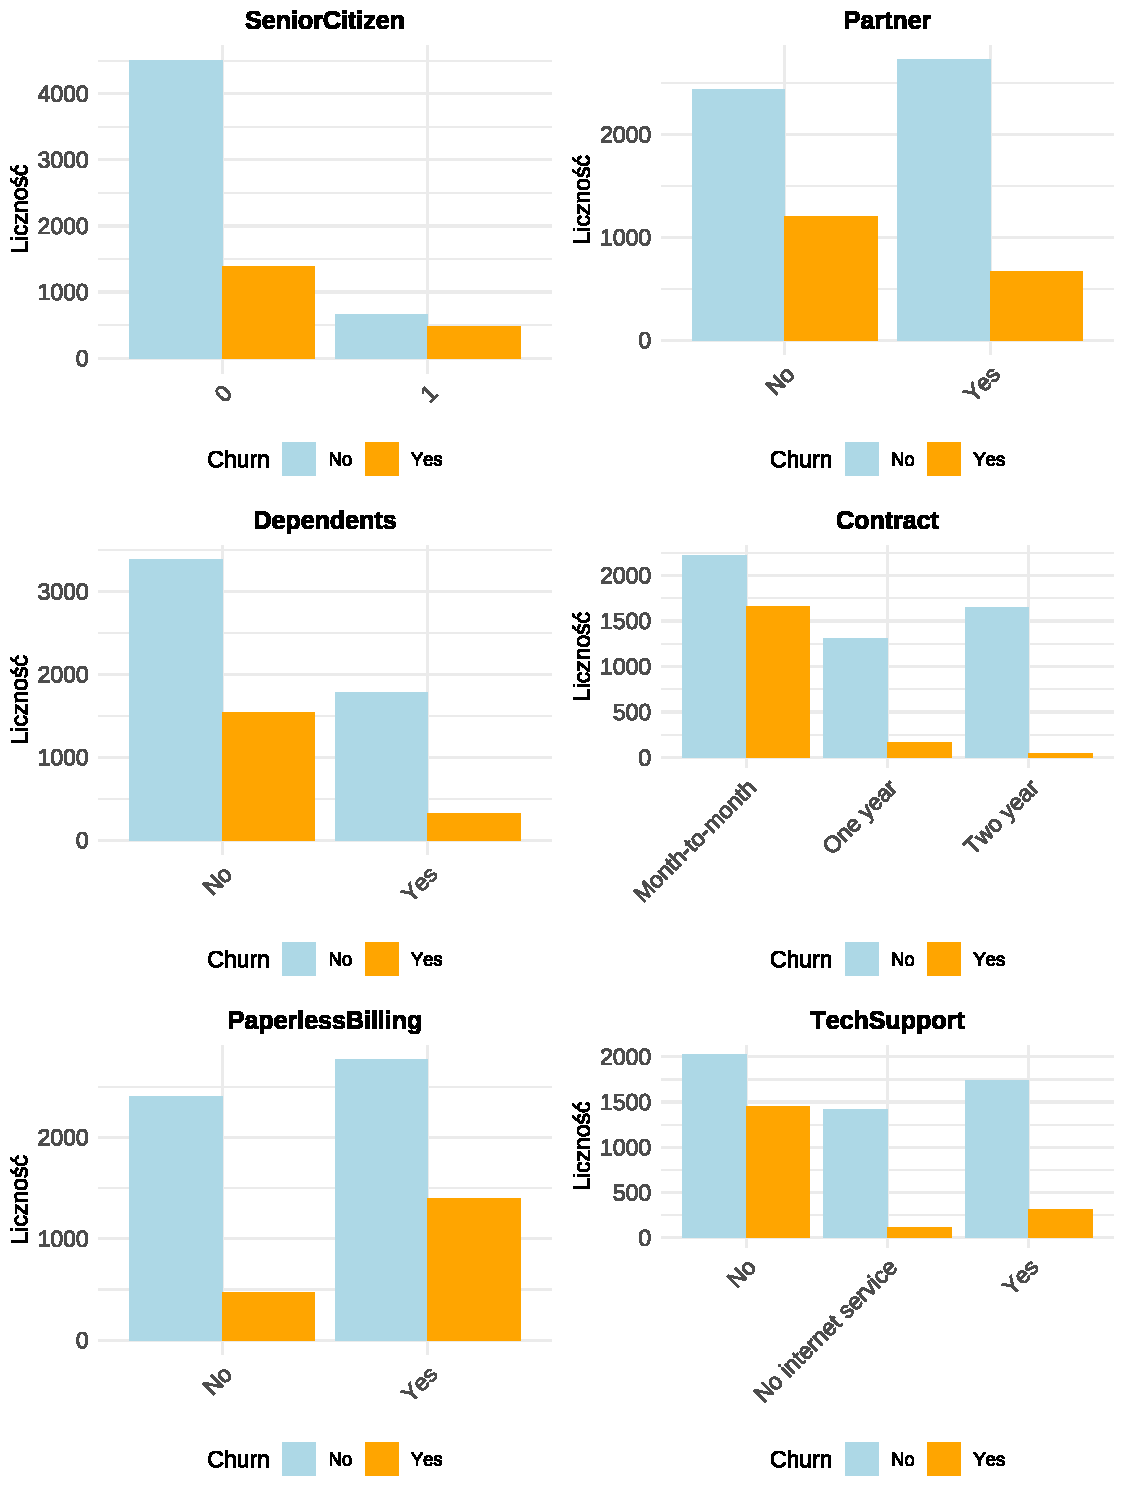
\includegraphics[width=0.85\textwidth]{figure/wykresy-slupkowe-churn-1} 

}

\caption{\label{fig:wykresy-slupkowe-churn} Wykresy słupkowe przedstawiające rozkład częstości wybranych zmiennych jakościowych z podziałem na grupy Churn}\label{fig:wykresy-slupkowe-churn}
\end{figure}

\end{knitrout}

\newpage
Analiza rozkładu zmiennych z podziałem na grupy Churn (Rysunek \ref{fig:wykresy-slupkowe-churn}) w połączeniu z danymi z tabel (Tabele: \ref{tab:churn_SeniorCitizen}, \ref{tab:churn_Partner}, \ref{tab:churn_Dependents}, \ref{tab:churn_Contract}, \ref{tab:churn_PaperlessBilling}, \ref{tab:churn_TechSupport}) ujawnia zależności:

\begin{itemize}
  \item \texttt{Contract:} Widoczna jest silna zależność między typem umowy a rezygnacją z usług (Tabela \ref{tab:churn_Contract}). Klienci z umowami miesięcznymi znacznie częściej rezygnują z usług (około 42\% przypadków) w porównaniu do tych z umowami dwuletnimi (jedynie około 11\% rezygnacji)
  
  \item \texttt{SeniorCitizen:} Jak pokazuje Tabela \ref{tab:churn_SeniorCitizen}, seniorzy, mimo że stanowią mniejszą część klientów, wykazują proporcjonalnie wyższy wskaźnik rezygnacji - około 41\% seniorów rezygnuje z usług, podczas gdy wśród pozostałych klientów odsetek ten wynosi około 24\%
  
  \item \texttt{PaperlessBilling:} Z danych w Tabeli \ref{tab:churn_PaperlessBilling} wynika, że klienci korzystający z e-faktur częściej rezygnują z usług (około 33\%) w porównaniu do klientów preferujących tradycyjne faktury (około 17\%), co może wskazywać na ich większą aktywność w poszukiwaniu lepszych ofert
  
  \item \texttt{Partner/Dependents:} Tabele \ref{tab:churn_Partner} i \ref{tab:churn_Dependents} pokazują, że osoby bez partnerów (około 31\% rezygnacji) lub osób zależnych (około 30\% rezygnacji) wykazują tendencję do częstszego zrywania umowy niż osoby posiadające partnera (około 21\% rezygnacji) lub osoby zależne (około 20\% rezygnacji), co sugeruje, że zobowiązania rodzinne mogą skłaniać do pozostania przy obecnym dostawcy usług
  
  \item \texttt{TechSupport:} Tabela \ref{tab:churn_TechSupport} ujawnia, że klienci bez wsparcia technicznego mają znacznie wyższy wskaźnik rezygnacji (około 40\%) w porównaniu do klientów korzystających z tej usługi (około 15\%), co sugeruje, że dobrze funkcjonujące wsparcie techniczne może być kluczowym czynnikiem utrzymania klientów
\end{itemize}


\subsubsection{Zmienne najlepiej rozróżniające grupy klientów rezygnujących i pozostających}

Przeprowadzona analiza danych z podziałem na grupy klientów, którzy zrezygnowali z usług (\texttt{Churn = Yes}) oraz tych, którzy pozostali (\texttt{Churn = No}), pozwala wyciągnąć następujące wnioski dotyczące zmiennych najlepiej rozróżniających te grupy:

\begin{enumerate}
  \item \texttt{Contract} - zmienna ta wykazuje najsilniejsze zróżnicowanie między grupami. Klienci z umowami miesięcznymi rezygnują z usług ponad trzykrotnie częściej (ok. 42\%) niż klienci z umowami dwuletnimi (ok. 11\%)
  
  \item \texttt{TechSupport} - dostęp do wsparcia technicznego istotnie wpływa na utrzymanie klienta. Osoby bez wsparcia technicznego rezygnują znacznie częściej (ok. 40\%) niż klienci korzystający z tej usługi (ok. 15\%)

\end{enumerate}



\newpage
\section{Podsumowanie - wnioski z przeprowadzonej analizy}

\subsection{Podsumowanie wyników}
Przeprowadzona analiza eksploracyjna danych klientów firmy telekomunikacyjnej wykazała, że zbiór danych zawiera 7043 obserwacje z 21 zmiennymi opisującymi klientów oraz zakres usług, z których korzystają. Analiza jednowymiarowa ujawniła nierównomierne rozkłady w kilku zmiennych, w szczególności przewagę umów miesięcznych oraz niski udział seniorów wśród klientów. Poziom rezygnacji klientów (\texttt{Churn}) wynosi około 26,5\%, co wskazuje na istotny problem zatrzymania klientów.

W analizie dwuwymiarowej zidentyfikowano kluczowe czynniki różnicujące klientów rezygnujących i pozostających. Zmienne jakościowe \texttt{Contract}, \texttt{TechSupport}, \texttt{SeniorCitizen} oraz \texttt{PaperlessBilling} wykazały najsilniejsze zależności ze zmienną \texttt{Churn}. Wśród zmiennych ilościowych największe różnice między grupami obserwujemy dla zmiennych \texttt{tenure} (długość korzystania z usług) oraz \texttt{MonthlyCharges} (miesięczne opłaty).

\subsection{Charakterystyka klientów firmy}
Klienci analizowanej firmy telekomunikacyjnej charakteryzują się następującymi cechami:
\begin{itemize}
  \item Przeważającą część stanowią osoby młodsze, nie będące seniorami (około 84\%)
  \item Liczba klientów posiadających i nieposiadających partnerów jest zbliżona (około 50\% do 50\%)
  \item Większość klientów nie posiada osób zależnych (około 70\%)
  \item Dominują klienci z umowami miesięcznymi (około 55\%), podczas gdy umowy jedno- i dwuletnie stanowią mniejszość
  \item Większość klientów posiada elektroniczne faktury (około 59\%)
  \item Znacząca część klientów nie korzysta z usług wsparcia technicznego
  \item Przeciętny czas korzystania z usług (\texttt{tenure}) wynosi około 32 miesięcy, przy czym wielu klientów korzysta z usług krócej niż rok
  \item Średnie miesięczne opłaty (\texttt{MonthlyCharges}) wynoszą około 65 dolarów, a ich rozkład jest dość równomierny
  \item Całkowite opłaty (\texttt{TotalCharges}) silnie korelują z czasem korzystania z usług i wykazują znaczne zróżnicowanie wśród klientów
\end{itemize}

\subsection{Główne przyczyny odchodzenia klientów i rekomendacje}
Na podstawie przeprowadzonych analiz można wskazać następujące główne przyczyny odchodzenia klientów:

\begin{enumerate}
  \item \textbf{Krótki czas korzystania z usług} - klienci o krótszym stażu (\texttt{tenure}) znacznie częściej rezygnują z usług, co wskazuje na kluczowy okres pierwszych 12 miesięcy dla utrzymania klienta
  \item \textbf{Wyższe miesięczne opłaty} - klienci płacący wyższe miesięczne rachunki (\texttt{MonthlyCharges}) mają tendencję do częstszej rezygnacji z usług
  \item \textbf{Rodzaj umowy} - klienci z umowami miesięcznymi rezygnują trzykrotnie częściej (42\%) niż klienci z umowami dwuletnimi (11\%)
  \item \textbf{Brak wsparcia technicznego} - klienci bez tej usługi rezygnują znacznie częściej (40\%) niż klienci z dostępem do wsparcia (15\%)
  \item \textbf{Status seniora} - seniorzy rezygnują częściej (41\%) niż młodsi klienci (24\%)
  \item \textbf{Elektroniczne faktury} - klienci korzystający z e-faktur częściej rezygnują (33\%) niż klienci preferujący tradycyjne faktury (17\%)
  \item \textbf{Brak zobowiązań rodzinnych} - osoby bez partnera oraz bez osób zależnych częściej rezygnują z usług
\end{enumerate}

\textbf{Rekomendacje dla firmy:}
\begin{itemize}
  \item Wdrożenie specjalnych programów dla nowych klientów
  \item Wprowadzenie zachęt do podpisywania długoterminowych umów
  \item Ulepszenie i automatyczne włączenie wsparcia technicznego jako standardowej usługi, szczególnie dla seniorów
  \item Opracowanie specjalnych pakietów dla seniorów
  \item Wprowadzenie programu lojalnościowego dla klientów korzystających z e-faktur, aby zrównoważyć ich większą skłonność do zmiany dostawcy
  \item Stworzenie dedykowanych planów rodzinnych z dodatkowymi korzyściami, aby zwiększyć lojalność klientów z zobowiązaniami rodzinnymi
\end{itemize}



\end{document}
